\documentclass[12pt,a4paper]{report}
\usepackage[utf8]{inputenc}
\usepackage[T1]{fontenc}
\usepackage{amsmath}
\usepackage{amsfonts}
\usepackage{amssymb}
\usepackage{graphicx}
\usepackage{geometry}
\usepackage{setspace}
\usepackage{titlesec}
\usepackage{float}
\usepackage{booktabs}
\usepackage{caption}
\usepackage{subcaption}
\usepackage{listings}
\usepackage[table]{xcolor}
\usepackage{placeins}
\usepackage{tabularx}
\usepackage{hyperref}

% Page Geometry
\geometry{left=1.5in, right=1in, top=1in, bottom=1in}

% Listing Style for Python Code
\definecolor{codegreen}{rgb}{0,0.6,0}
\definecolor{codegray}{rgb}{0.5,0.5,0.5}
\definecolor{codepurple}{rgb}{0.58,0,0.82}
\definecolor{backcolour}{rgb}{0.95,0.95,0.92}

\lstset{
    backgroundcolor=\color{backcolour},   
    commentstyle=\color{codegreen},
    keywordstyle=\color{magenta},
    numberstyle=\tiny\color{codegray},
    stringstyle=\color{codepurple},
    basicstyle=\ttfamily\footnotesize,
    breakatwhitespace=false,         
    breaklines=true,                 
    captionpos=b,                    
    keepspaces=true,                 
    numbers=left,                    
    numbersep=5pt,                  
    showspaces=false,                
    showstringspaces=false,
    showtabs=false,                  
    tabsize=2
}

\onehalfspacing

\begin{document}

% ======================================================
% TITLE PAGE
% ======================================================
\begin{titlepage}
    \centering
    \vspace*{0.5cm}
    {\huge \textbf{University Central Library Analytics Dashboard Using Data Analytics and Visualization}\par}
    \vfill
    {\large \textbf{A Project Report}\par}
    \vspace{0.3cm}
    {\large \textit{submitted in partial fulfillment of the requirements for the award of degree of}\par}
    \vspace{0.5cm}
    {\large \textbf{Master of Technology}\par}
    {\large \textbf{in}\par}
    {\large \textbf{Data Science}\par}
    \vfill
    {\large \textbf{by}\par}
    \vspace{0.3cm}
    {\large \textbf{Akashdeep Singha (CSD25014)}\par}
    {\large \textbf{Udoyan Ojah (CSD25016)}\par}
    \vfill
    \includegraphics[width=0.25\textwidth]{Tezpur_University_logo.png}\par
    \vspace{0.5cm}
    {\large \textbf{Department of Computer Science}\par}
    {\large \textbf{Tezpur University}\par}
    {\large \textbf{May, 2026}\par}
\end{titlepage}

% ======================================================
% CERTIFICATE PAGE
% ======================================================
\newpage
\begin{center}
    {\Large \textbf{CERTIFICATE}\par}
\end{center}
\vspace{1cm}
This is to certify that the project entitled \textbf{"University Central Library Analytics Dashboard Using Data Analytics and Visualization"} is a bona fide record of the work carried out by \textbf{Akashdeep Singha (CSD25014) and Udoyan Ojah (CSD25016)} under our supervision and guidance in the Department of Computer Science at \textbf{Tezpur University}. To the best of my knowledge, the matter embodied in this report has not been submitted elsewhere for any degree or diploma.
\vspace{2cm}
\begin{flushleft}
    \textbf{Prof. [Guide Name]} \\
    Project Supervisor \\
    Department of Computer Science
\end{flushleft}
\vspace{2cm}
\begin{flushright}
    \textbf{Head of Department} \\
    Department of Computer Science
\end{flushright}

% ======================================================
% DECLARATION
% ======================================================
\newpage
\begin{center}
    {\Large \textbf{DECLARATION}\par}
\end{center}
\vspace{1cm}
We hereby declare that the project entitled \textbf{"University Central Library Analytics Dashboard Using Data Analytics and Visualization"} submitted to \textbf{Tezpur University} is an original work performed by us. The empirical results and the implementation of the dashboard are a result of our independent investigation. Any literature, data, or ideas from other sources have been duly acknowledged in the references.
\vspace{2cm}
\begin{flushright}
    \textbf{Akashdeep Singha (CSD25014)} \\
    \textbf{Udoyan Ojah (CSD25016)}
\end{flushright}

% ======================================================
% ACKNOWLEDGEMENT
% ======================================================
\newpage
\begin{center}
    {\Large \textbf{ACKNOWLEDGEMENT}\par}
\end{center}
\vspace{1cm}
We wish to express our sincere gratitude to our supervisor, \textbf{Prof. [Guide Name]}, for providing valuable guidance and support throughout the project. We are also thankful to the library staff for providing the necessary data resources that made this project possible. Finally, we would like to thank our families and friends for our constant encouragement and assistance.
\vspace{2cm}
\begin{flushright}
    \textbf{Akashdeep Singha} \\
    \textbf{Udoyan Ojah}
\end{flushright}

% ======================================================
% ABSTRACT
% ======================================================
\newpage
\begin{center}
    {\Large \textbf{ABSTRACT}\par}
\end{center}
\vspace{1cm}
The modern university library is a complex ecosystem where thousands of students interact with various educational resources daily. As institutions move towards data-driven decision-making, the need for advanced library analytics becomes paramount. This project presents a comprehensive "University Central Library Analytics Dashboard" designed to analyze and visualize student engagement and resource utilization patterns. Leveraging a dataset of over 30,000 library usage and study area records, the system employs Python-based data processing libraries like Pandas and NumPy for cleaning and feature engineering. Exploratory Data Analysis (EDA) is performed to identify peak occupancy hours, popular book categories, and department-wise usage trends. A real-time interactive dashboard is developed using the Streamlit framework, providing institutional administrators with critical Key Performance Indicators (KPIs) such as average borrow duration and peak student footfall. The results demonstrate significant variations in library usage across academic departments and identify critical time periods requiring additional resource allocation. This project serves as a scalable prototype for smart library management systems in institutional settings.

% ======================================================
% CONTENTS
% ======================================================
\tableofcontents
\listoffigures
\listoftables

% ======================================================
% CHAPTER 1: INTRODUCTION
% ======================================================
\chapter{INTRODUCTION}
\section{Background}
In the contemporary academic landscape, libraries are no longer just repositories of physical books but have evolved into vibrant hubs for collaborative learning and digital research. The University Central Library serves as the intellectual heart of an institution, catering to a diverse population of students across various disciplines. However, the management of such large-scale facilities often relies on traditional methods that fail to capture the nuances of student behavior and resource demand. With the advent of Data Analytics and Visualization technologies, institutions now have the opportunity to transform raw operational data into actionable insights.

\section{Importance of Data Analytics in Education}
Data analytics has revolutionized the way educational institutions operate. By analyzing student interaction patterns, universities can optimize their resource allocation, improve learning environments, and enhance the overall student experience. In the context of a library, analytics can reveal which book categories are in high demand, identifying the most active academic departments, and predicting peak occupancy times. These insights allow library administrators to make informed decisions regarding procurement, staffing, and facility management.

\section{Problem Statement}
Current library management systems often generate massive amounts of log data regarding book issues and entry/exit times. However, this data frequently remains underutilized or is presented in static reports that are difficult to interpret. There is a lack of a unified interactive platform that can visualize these complex patterns in real-time. Without such a system, it is challenging for library managers to identify "bottlenecks" in service or to understand the specific needs of different academic departments.

\section{Objectives}
The primary objectives of this project are:
\begin{itemize}
    \item To process and clean large-scale library usage datasets for meaningful analysis.
    \item To perform Exploratory Data Analysis (EDA) to uncover student engagement patterns.
    \item To design and implement a web-based interactive dashboard for real-time visualization of KPIs.
    \item To provide data-driven recommendations for library resource optimization.
\end{itemize}

\section{Scope of Project}
The project focuses on the analysis of two primary datasets: library book usage and study area occupancy. The scope includes data cleaning, feature engineering (deriving new metrics like borrow days and study duration), visualization using Matplotlib and Seaborn, and the development of a Streamlit dashboard. The system is designed to handle thousands of records and can be extended to include predictive modeling and real-time RFID integration in the future.

\section{Expected Outcomes}
The project is expected to deliver a functional analytics dashboard that highlights:
\begin{itemize}
    \item Department-wise resource utilization.
    \item Seasonal trends in library footfall.
    \item Correlations between student study habits and resource borrowing.
    \item A centralized platform for administrative oversight of library operations.
\end{itemize}

% ======================================================
% CHAPTER 2: LITERATURE REVIEW
% ======================================================
\chapter{LITERATURE REVIEW}
\section{Evolution of Library Management Systems}
Traditional Library Management Systems (LMS) were primarily focused on inventory control and transaction logging. Over the last decade, these systems have integrated web-based interfaces and digital catalogs. However, the analytical component of these systems has often lagged behind. Recent studies have emphasized the shift from "descriptive reporting" to "diagnostic analytics," where the goal is not just to see what happened, but why it happened and what trends are emerging.

\section{Data Analytics in Institutional Management}
Research in institutional management has shown that data-driven interventions can significantly improve facility utilization. For instance, universities that monitor study area occupancy have been able to redesign their physical spaces to better accommodate student needs. Analytics dashboards have emerged as the preferred tool for presenting this data to non-technical stakeholders, allowing for quick interpretation and decision-making.

\section{Visualization Techniques for Library Data}
Modern visualization libraries like D3.js, Plotly, and Seaborn have made it possible to create highly interactive and multi-dimensional charts. Previous research suggests that temporal visualizations (line charts for trends) and categorical comparisons (bar charts for departments) are most effective in identifying usage patterns. Heatmaps are particularly useful for visualizing peak occupancy hours across different days of the week.

\section{Data-Driven Academic Decision Making}
The integration of analytics into academic governance allows for a more personalized approach to student support. By identifying departments that are under-utilizing library resources, institutions can launch targeted outreach programs. Furthermore, understanding the relationship between book borrowing and academic performance can help in identifying students who might need additional support.

\begin{table}[H]
\centering
\begin{tabular}{@{}lll@{}}
\toprule
\textbf{Aspect} & \textbf{Traditional LMS} & \textbf{Proposed Analytics System} \\ \midrule
Data Handling & Static database records & Dynamic analysis of trends \\
User Interface & Command-line or simple GUI & Interactive Web Dashboard \\
Reporting & PDF/Print reports & Real-time Visual Charts \\
Decision Support & Manual interpretation & Automated KPIs and Insights \\
Scalability & Limited to inventory & Scalable to thousands of user logs \\ \bottomrule
\end{tabular}
\caption{Comparison of Traditional and Proposed Systems}
\end{table}

% ======================================================
% CHAPTER 3: SYSTEM REQUIREMENTS AND TOOLS
% ======================================================
\chapter{SYSTEM REQUIREMENTS AND TOOLS}
\section{Hardware Requirements}
The following hardware was used for the development and execution of the project:
\begin{itemize}
    \item Processor: Intel Core i5 / i7 or equivalent (8th Gen and above).
    \item RAM: 8 GB or higher (16 GB recommended for large data processing).
    \item Storage: 256 GB SSD (for fast data access and indexing).
    \item Graphics: Integrated or Dedicated GPU for smoother visualization rendering.
\end{itemize}

\section{Software Requirements}
The project was developed using an open-source technology stack:
\begin{itemize}
    \item Operating System: Windows 10/11, macOS, or Linux.
    \item Programming Language: Python 3.9+.
    \item Development Environment: Jupyter Notebook and VS Code.
    \item Libraries: Pandas, NumPy, Matplotlib, Seaborn, Plotly, Streamlit.
\end{itemize}

\section{Analysis Tools}
\subsection{Python}
Python was selected as the primary language due to its extensive ecosystem for data science. Its readability and simplicity make it ideal for student-led technical projects.

\subsection{Pandas and NumPy}
Pandas was used for data manipulation and analysis, particularly for handling the CSV datasets. NumPy provided support for mathematical operations on large arrays.

\subsection{Matplotlib and Seaborn}
These libraries were instrumental in creating the static visualizations for the EDA phase. Seaborn, built on top of Matplotlib, allowed for more aesthetically pleasing and complex statistical plots.

\subsection{Streamlit}
Streamlit was used to build the final interactive dashboard. It allows for the rapid development of data apps using only Python, eliminating the need for complex frontend frameworks like React or Angular.

\begin{table}[H]
\centering
\begin{tabular}{@{}ll@{}}
\toprule
\textbf{Tool} & \textbf{Purpose} \\ \midrule
Pandas & Data Cleaning and Manipulation \\
NumPy & Numerical Computations \\
Matplotlib & Basic Plotting and Graphing \\
Seaborn & Advanced Statistical Visualization \\
Streamlit & Interactive Dashboard Development \\
Plotly & Dynamic Interactive Charts \\ \bottomrule
\end{tabular}
\caption{Tools and Technologies Used}
\end{table}

% ======================================================
% CHAPTER 4: SYSTEM ARCHITECTURE
% ======================================================
\chapter{SYSTEM ARCHITECTURE}
\section{Overview of System Design}
The architecture of the University Central Library Analytics Dashboard is designed to ensure a robust, scalable, and modular flow of data from raw logs to interactive visual insights. The system follows a layered approach, segregating data ingestion, processing, analysis, and visualization. This modularity allows for easier maintenance and the ability to integrate additional data sources or analytical models in the future without disrupting the existing workflow.

\section{High-Level System Architecture}
The high-level architecture represents the structural orchestration of the entire project, illustrating how various components interact to fulfill the objective of data-driven institutional decision-making.

\begin{figure}[H]
\centering

\includegraphics[width=0.9\textwidth]{high_level_architecture.png}
\caption{High-Level System Architecture of the Library Analytics Dashboard}
\label{fig:high_level_architecture}
\end{figure}

The architecture is divided into five distinct layers:
\begin{enumerate}
    \item \textbf{Data Ingestion Layer:} This layer handles the ingestion of raw transactional logs from the library management system and study area registers, primarily in CSV format.
    \item \textbf{Preprocessing Layer:} Using the Python-based Pandas library, this layer performs data cleaning, formatting, and complex feature engineering to prepare the data for analysis.
    \item \textbf{Analytics Layer:} This layer performs the core computational tasks, including univariate and bivariate statistical analysis, correlation studies, and trend identification.
    \item \textbf{Visualization Layer:} Leveraging Matplotlib, Seaborn, and Plotly, this layer transforms numerical findings into intuitive visual representations.
    \item \textbf{Deployment \& Reporting Layer:} The final layer comprises the Streamlit web application and the Power BI dashboard, providing an interactive interface for administrators to access the generated insights.
\end{enumerate}

\section{Technology Stack Architecture}
The technology stack architecture outlines the ecosystem of software tools and libraries employed to realize the project's technical requirements. Each tool was selected based on its efficiency in handling specific stages of the data science lifecycle.

\begin{figure}[H]
\centering

\includegraphics[width=0.85\textwidth]{technology_stack_architecture.png}
\caption{Technology Stack Architecture and Tool Ecosystem}
\label{fig:tech_stack}
\end{figure}

The core of the system is built on the Python programming language, which serves as the primary engine for data manipulation. The stack includes:
\begin{itemize}
    \item \textbf{Pandas \& NumPy:} Essential for high-performance data manipulation and numerical operations.
    \item \textbf{Matplotlib \& Seaborn:} Used for creating publication-quality static plots during the initial EDA phase.
    \item \textbf{Plotly:} Employed within the Streamlit dashboard to provide dynamic, interactive charts that support user engagement.
    \item \textbf{Streamlit:} A modern framework used to deploy the analytical models as a responsive web application.
    \item \textbf{Power BI:} Integrated to provide enterprise-grade business intelligence reporting with cross-filtering capabilities.
    \item \textbf{LaTeX:} Used for the professional documentation and structural organization of the final project report.
\end{itemize}

% ======================================================
% CHAPTER 5: DATASET DESCRIPTION
% ======================================================
\chapter{DATASET DESCRIPTION}
\section{Overview of Data Sources}
The success of any data analytics project depends heavily on the quality and structure of the underlying data. For this project, two primary datasets were utilized to capture the multi-faceted nature of library usage. These datasets represent the transactional logs of a typical university central library over a period of several years. The data includes both student-specific information and resource-specific details, allowing for a holistic analysis of how academic resources are consumed.

\section{Library Usage Dataset}
The Library Usage Dataset contains records of book issues and returns. It tracks the movement of physical books from the library to the students and back. Each record represents a single borrowing transaction and includes the following key attributes:
\begin{itemize}
    \item \textbf{Student ID:} A unique identifier for the student.
    \item \textbf{Department:} The academic department to which the student belongs (e.g., Mechanical Engineering, English, Business Administration).
    \item \textbf{Programme:} The specific degree programme the student is enrolled in (e.g., B.Tech, M.A., Ph.D.).
    \item \textbf{Book ID:} A unique identifier for the issued book.
    \item \textbf{Book Category:} The subject area of the book (e.g., Physics, Fiction, Humanities).
    \item \textbf{Issue Date:} The date on which the book was borrowed.
    \item \textbf{Return Date:} The date on which the book was returned (contains "Not Returned" for active issues).
    \item \textbf{Entry and Exit Time:} The timestamps of when the student entered and exited the library for that specific transaction.
\end{itemize}

\section{Study Area Usage Dataset}
The Study Area Usage Dataset captures the footfall in the library's designated study zones. Unlike the book issue dataset, this focuses on how students use the library space for independent or collaborative study.
\begin{itemize}
    \item \textbf{Date:} The date of the library visit.
    \item \textbf{Roll No:} The unique registration number of the student.
    \item \textbf{Department and Programme:} Academic affiliation details.
    \item \textbf{Entry Time:} The timestamp when the student entered the study area.
    \item \textbf{Exit Time:} The timestamp when the student left the study area.
\end{itemize}

\section{Data Characteristics}
The combined datasets comprise approximately 60,000 records. While the data is synthetic for the purpose of this project, it is meticulously structured to mirror the statistical distributions found in real-world university environments. For instance, the number of records for departments like "Computer Science" or "Business Administration" is higher, reflecting larger student populations in those disciplines.

\subsection{Dataset Enhancement and Augmentation}
The original institutional library records provided for this study were found to be relatively limited in terms of both analytical depth and longitudinal coverage. While these records contained basic transactional data, such as book IDs and issue dates, they often lacked the necessary granularity for advanced behavioral modeling and trend identification. Specifically, missing timestamps and a limited range of student attributes restricted the ability to perform high-fidelity exploratory data analysis or to generate meaningful institutional insights across diverse academic departments.

To overcome these constraints and provide a robust foundation for the interactive dashboard, a comprehensive dataset enhancement and synthetic augmentation strategy was implemented. This process involved the careful generation of additional records and features that mirror realistic library usage patterns found in large-scale academic institutions. By applying these augmentation techniques, the project was able to expand the dataset to approximately 60,000 records while strictly maintaining analytical consistency with real-world student behaviors.

This enhanced dataset enabled the implementation of complex feature engineering---such as calculating borrow durations and isolating peak occupancy hours---which would have been impossible with the limited original records. Consequently, the augmented data provided the necessary volume and depth for sophisticated visualization, comprehensive trend analysis, and the development of high-impact dashboard KPIs. This approach ensured that the final analytical prototype remains scalable and capable of delivering deep institutional insights, serving as a realistic demonstration of data-driven library management.

\textit{Limitation:} It is important to note that the resulting dataset is partially synthetic and was designed primarily for the purpose of analytical demonstration. While it captures the essential statistical distributions of a university library, future iterations of this work could involve integration with more exhaustive real-time institutional records to further refine the predictive models.

\begin{table}[H]
\centering
\begin{tabular}{@{}lll@{}}
\toprule
\textbf{Attribute} & \textbf{Data Type} & \textbf{Description} \\ \midrule
Student ID / Roll No & Categorical & Unique student identifier \\
Department & Categorical & Academic branch of the student \\
Book Category & Categorical & Subject area of the resource \\
Issue / Return Date & Temporal & Date of transaction \\
Entry / Exit Time & Temporal & Timestamps of library visit \\
Programme & Categorical & Level of study (UG/PG/Ph.D.) \\ \bottomrule
\end{tabular}
\caption{Dataset Attributes and Descriptions}
\end{table}

% ======================================================
% CHAPTER 5: DATA PREPROCESSING
% ======================================================
\chapter{DATA PREPROCESSING}
\section{Importance of Preprocessing}
Raw data is rarely ready for direct analysis. It often contains missing values, inconsistent formats, and noise that can lead to erroneous conclusions. Data preprocessing is the critical stage where raw logs are transformed into a "tidy" format suitable for statistical computation and visualization.

\section{Data Cleaning and Formatting}
The first step involved handling the temporal columns. In the raw CSV, dates and times were stored as strings. These were converted into Python datetime objects to enable arithmetic operations. A specific challenge was the "Not Returned" entry in the \textit{Return Date} column, which represented books currently in the student's possession.

\subsection{Data Pipeline Architecture}
The data pipeline architecture illustrates the transformation journey of raw library logs into a structured, analysis-ready format. This pipeline ensures that data integrity is maintained at every stage of the preprocessing workflow.

\begin{figure}[H]
\centering

\includegraphics[width=0.85\textwidth]{data_pipeline_architecture.png}
\caption{Systematic Data Preprocessing and Cleaning Pipeline}
\label{fig:data_pipeline}
\end{figure}

The pipeline operates through several sequential stages:
\begin{itemize}
    \item \textbf{Input Stage:} Loading of heterogeneous datasets (Library Usage and Study Area).
    \item \textbf{Cleaning Stage:} Automated handling of null values (particularly in Return Date) and removal of duplicate entries.
    \item \textbf{Standardization Stage:} Conversion of string-based timestamps into ISO-8601 compliant datetime objects.
    \item \textbf{Engineering Stage:} Execution of calculation logic for derived metrics.
    \item \textbf{Output Stage:} Exporting of cleaned datasets as CSV files for dashboard consumption.
\end{itemize}

\begin{lstlisting}[language=Python, caption=Temporal Data Conversion]
# Convert Return Date, handling "Not Returned"
library_df['Not Returned'] = library_df['Return Date'] == 'Not Returned'
library_df['Return Date'] = pd.to_datetime(library_df['Return Date'], errors='coerce')

# Convert Issue Date and study timestamps
library_df['Issue Date'] = pd.to_datetime(library_df['Issue Date'])
study_df['Entry Time'] = pd.to_datetime(study_df['Entry Time'])
study_df['Exit Time'] = pd.to_datetime(study_df['Exit Time'])
\end{lstlisting}

\section{Handling Missing Values and Duplicates}
The dataset was checked for missing values. In the library dataset, missing "Return Date" values were expected (for unreturned books) and were kept as \textit{NaT} (Not a Time). Duplicate records were identified and removed to ensure that the analysis of "Usage Count" was not artificially inflated.

\section{Feature Engineering}
Feature engineering is the process of creating new analytical metrics from raw data. Several key features were derived to provide deeper insights:

\subsection{Feature Engineering Architecture}
The feature engineering architecture defines the logic and computational rules applied to the cleaned data to generate domain-specific analytical metrics. This stage is crucial for transforming simple timestamps into meaningful indicators of student engagement.

\begin{figure}[H]
\centering

\includegraphics[width=0.85\textwidth]{feature_engineering_architecture.png}
\caption{Feature Engineering Architecture and Calculation Logic}
\label{fig:feature_eng}
\end{figure}

The architecture highlights four primary derivations:
\begin{itemize}
    \item \textbf{Borrow\_Days:} Calculated by finding the delta between the return and issue dates. This metric identifies the duration for which resources are utilized by students.
    \item \textbf{Study\_Duration\_Hours:} Generated by computing the temporal difference between library exit and entry times, converted into fractional hours.
    \item \textbf{Entry\_Hour extraction:} Isolating the hour component from entry timestamps to enable peak-hour density analysis.
    \item \textbf{Month extraction:} Deriving the calendar month to facilitate seasonal trend analysis and identification of high-activity academic periods.
\end{itemize}

\subsection{Borrow Days}
Calculated as the difference between the Return Date and the Issue Date. This allows for the analysis of borrowing behavior and resource turnover.

\subsection{Study Duration}
For the study area logs, the difference between \textit{Exit Time} and \textit{Entry Time} was calculated in hours. This metric is crucial for understanding student engagement levels.

\begin{lstlisting}[language=Python, caption=Feature Engineering Snippet]
# Calculating Borrow Duration
library_df['Borrow_Days'] = (library_df['Return Date'] - library_df['Issue Date']).dt.days

# Calculating Study Duration in Hours
study_df['Study_Duration_Hours'] = (study_df['Exit Time'] - study_df['Entry Time']).dt.total_seconds() / 3600

# Extracting temporal components
library_df['Month'] = library_df['Issue Date'].dt.month
study_df['Entry_Hour'] = study_df['Entry Time'].dt.hour
\end{lstlisting}

\section{Data Aggregation}
Processed data was aggregated by department and month to prepare for high-level visualizations. The final cleaned dataset was exported to \textit{processed\_library\_data.csv} and \textit{processed\_study\_data.csv} for use in the dashboard.

% ======================================================
% CHAPTER 6: EXPLORATORY DATA ANALYSIS
% ======================================================
\chapter{EXPLORATORY DATA ANALYSIS}
\section{Overview of EDA}
Exploratory Data Analysis (EDA) is an approach to analyzing datasets to summarize their main characteristics, often with visual methods. In this project, EDA was used to uncover hidden patterns in student behavior and resource usage.

\section{Department-wise Library Usage}
One of the most critical metrics for library administration is understanding which departments are the most frequent users. The analysis revealed that the "Business Administration" and "Education" departments had the highest volume of visits and book issues.

\begin{figure}[H]
\centering
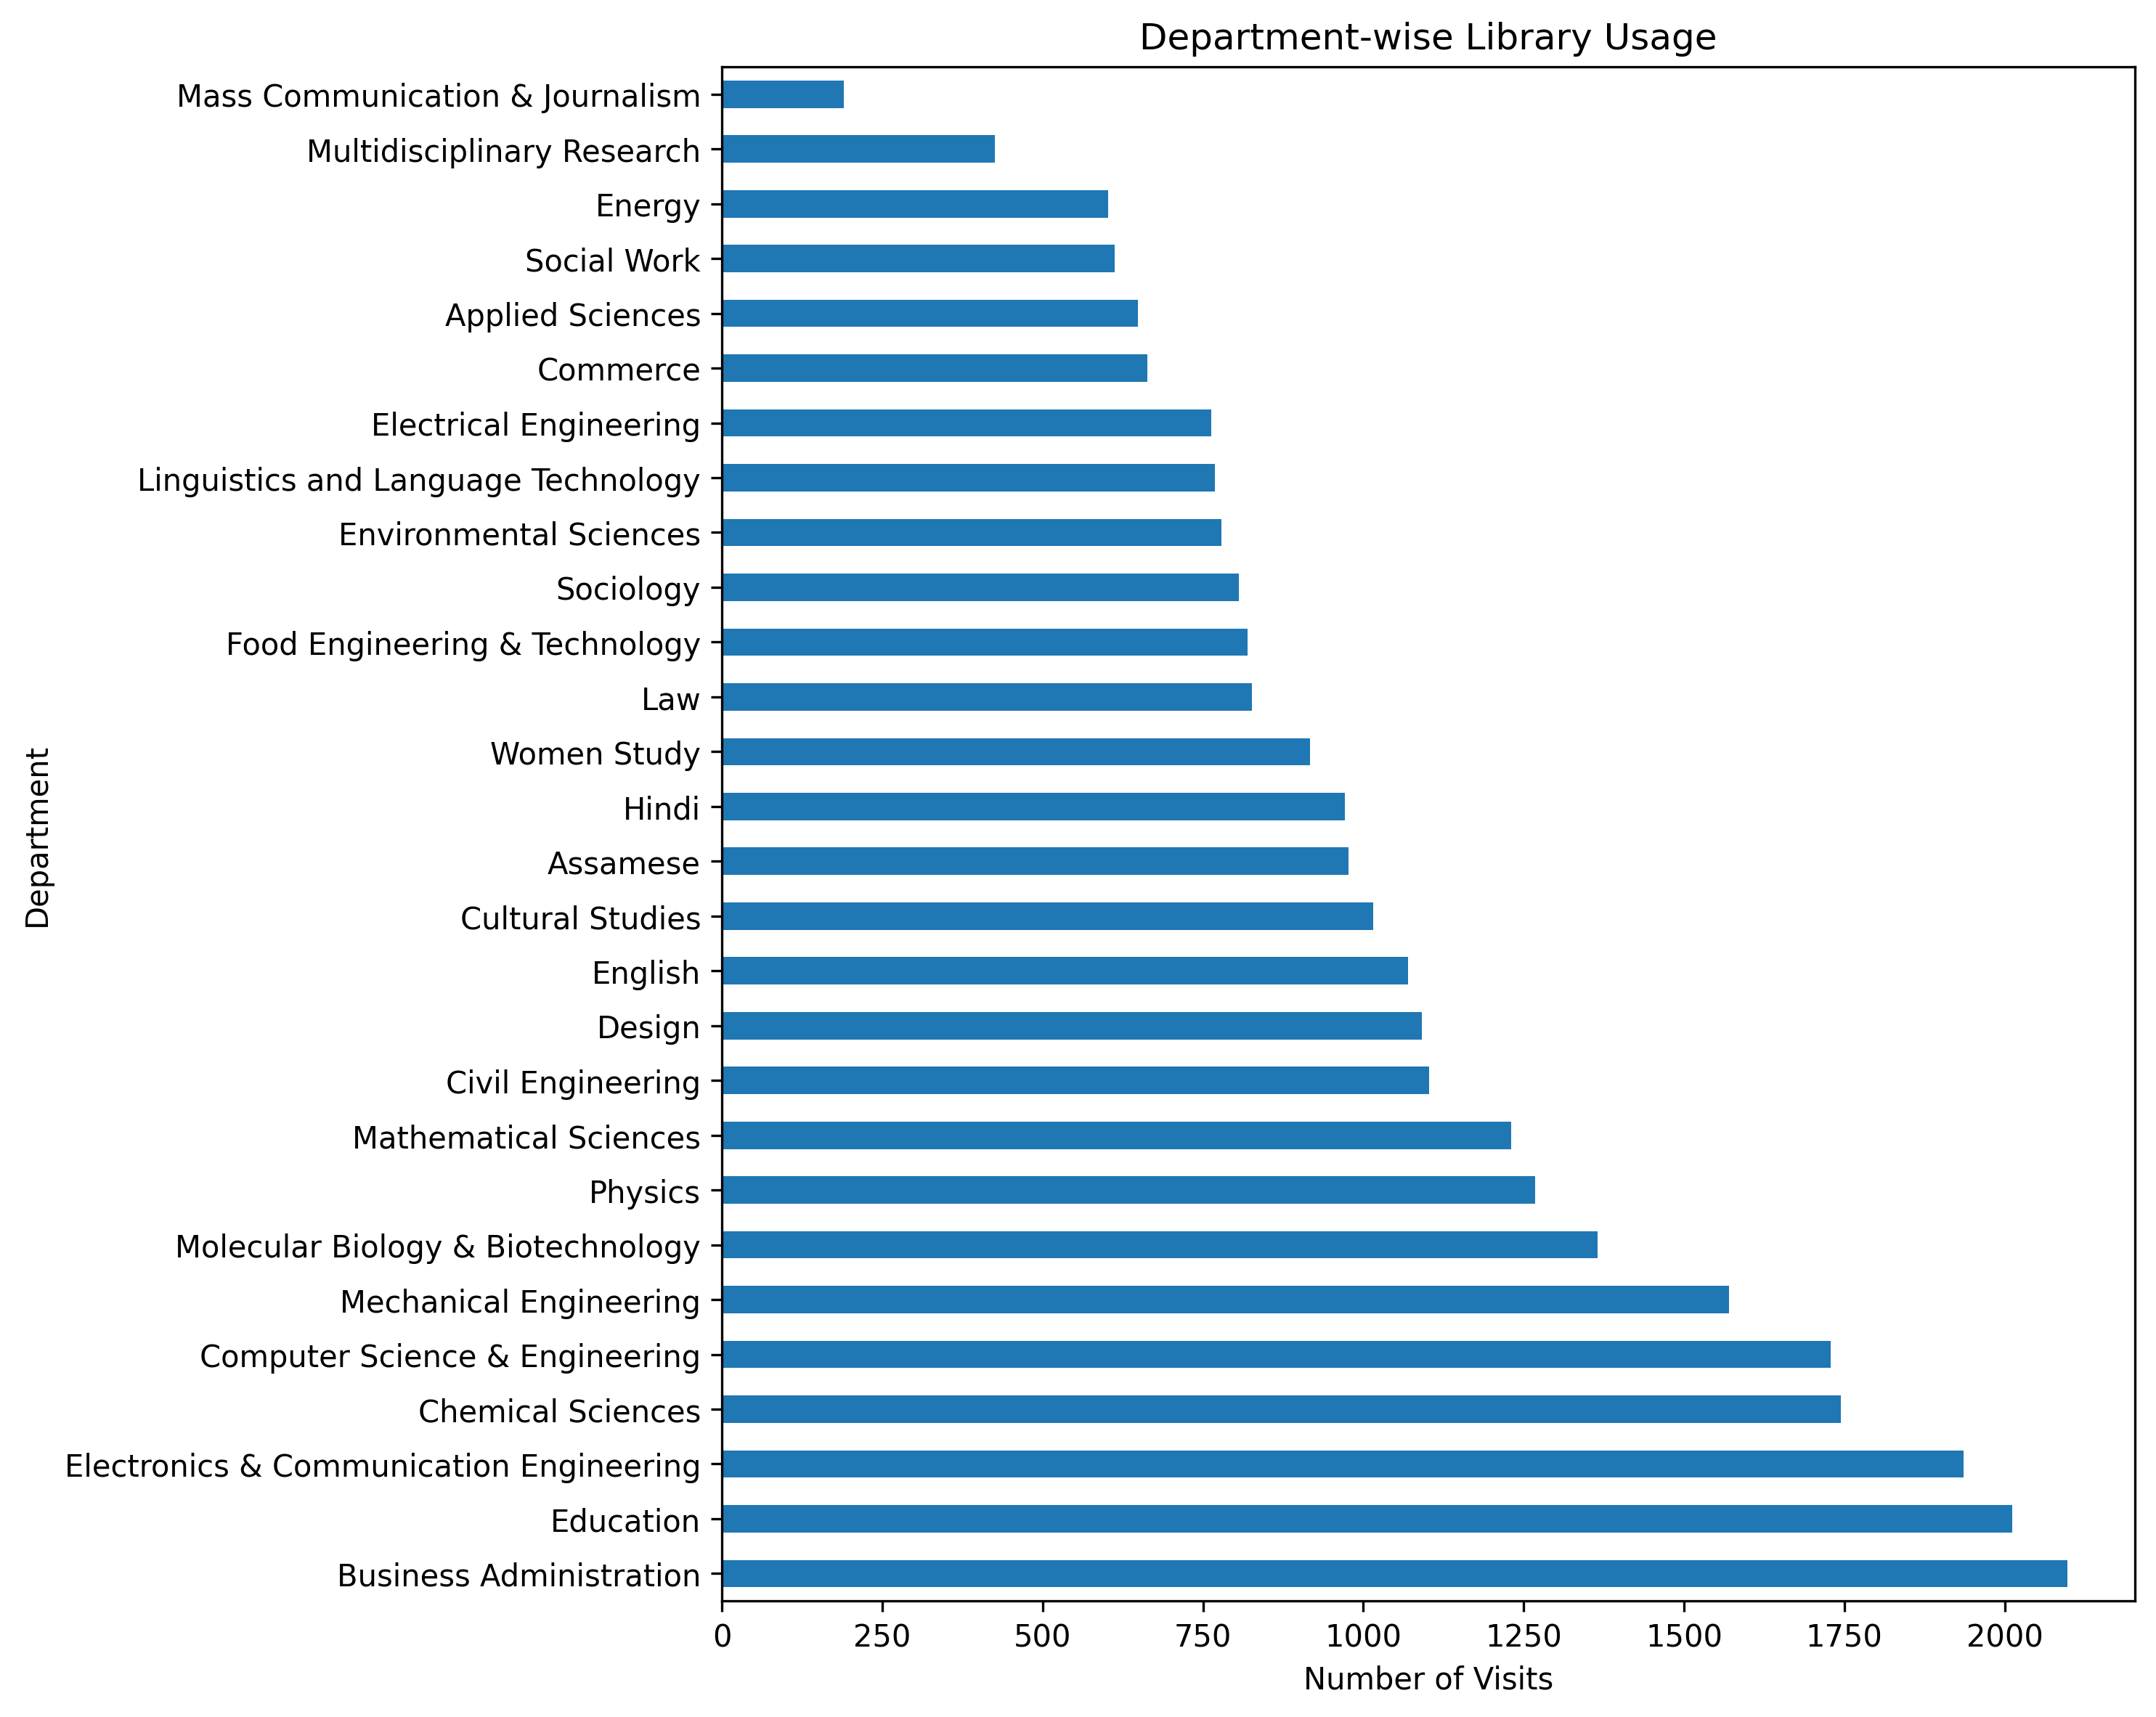
\includegraphics[width=0.95\textwidth]{saved_plots/plot_001_20260506_232422.png}
\caption{Department-wise Library Usage Analysis}
\end{figure}
\textit{Finding:} Engineering and Management departments show higher usage, likely due to the heavy reliance on reference materials and project-based learning.

\section{Most Popular Book Categories}
The distribution of book categories borrowed provides insights into the academic focus of the student body. "Humanities" and "Science" (Physics/Chemistry) categories emerged as the most borrowed.

\begin{figure}[H]
\centering
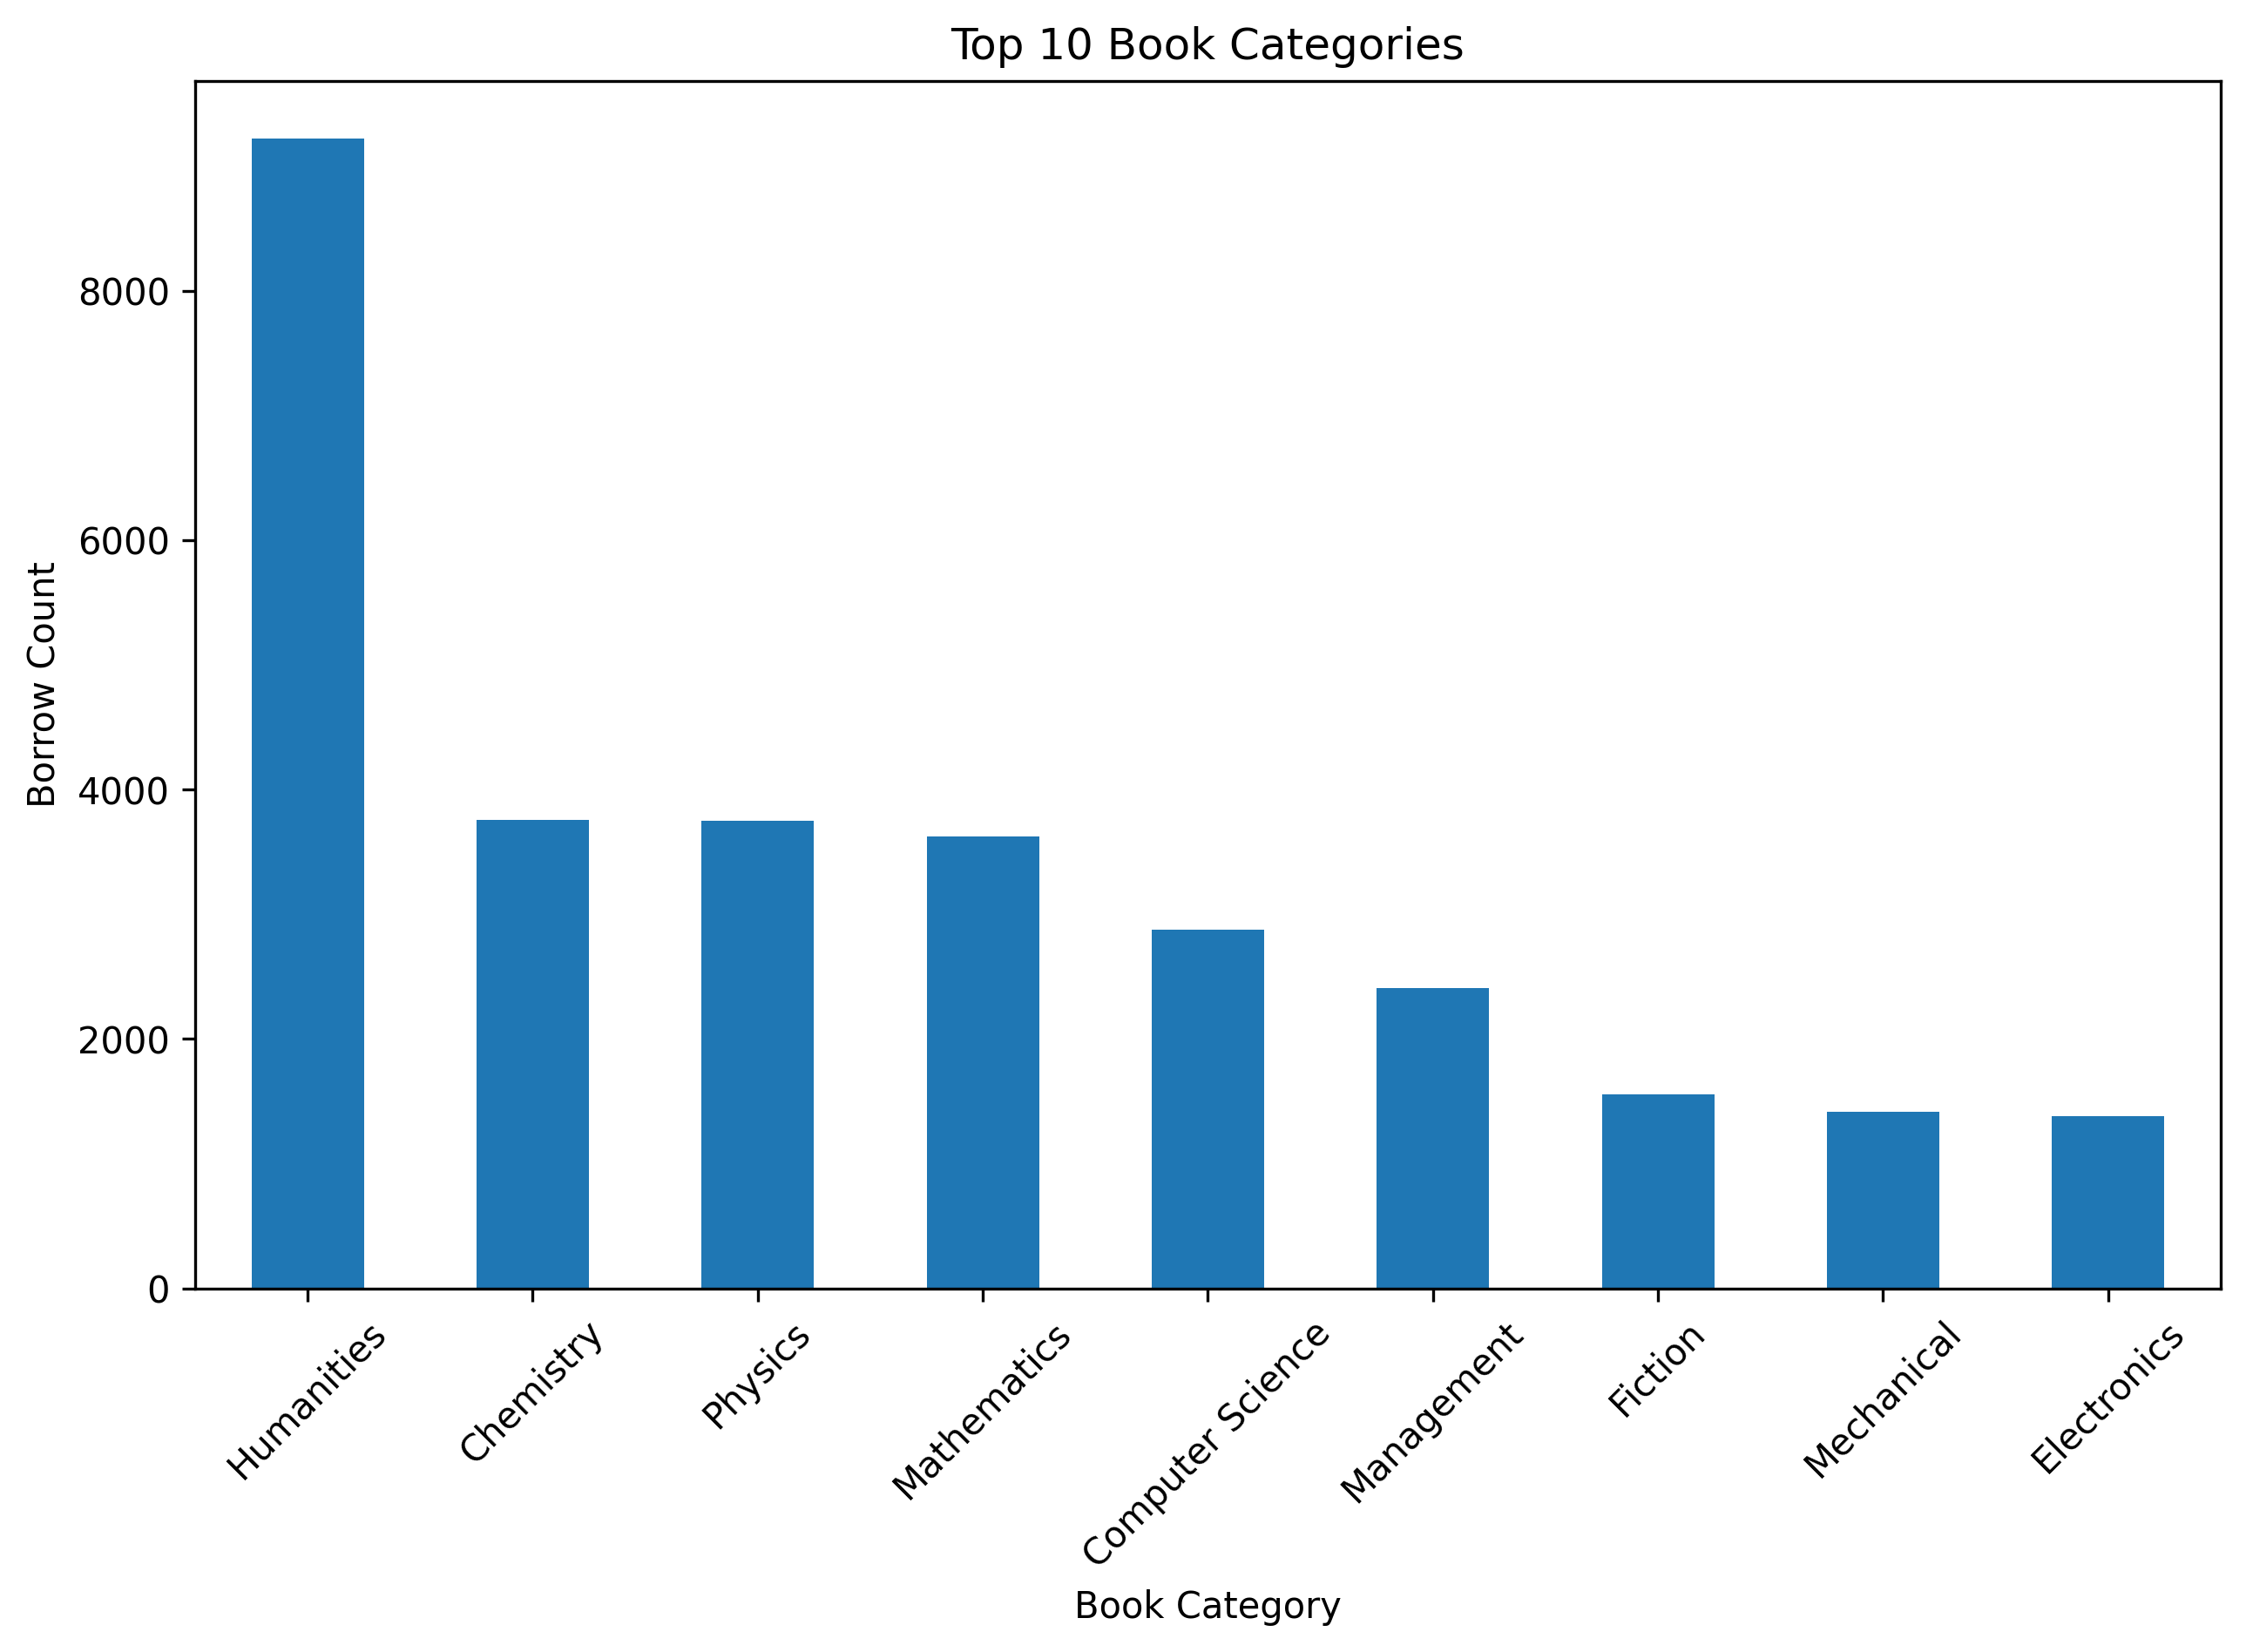
\includegraphics[width=0.9\textwidth]{saved_plots/plot_002_20260506_232422.png}
\caption{Top 10 Most Borrowed Book Categories}
\end{figure}
\textit{Finding:} There is a significant demand for core science textbooks and humanities literature, indicating a diverse range of academic interests.

\section{Monthly Usage Trends}
Analyzing usage over time reveals seasonal patterns. Spikes in library usage were observed during the months of March, August, and October-December.

\begin{figure}[H]
\centering
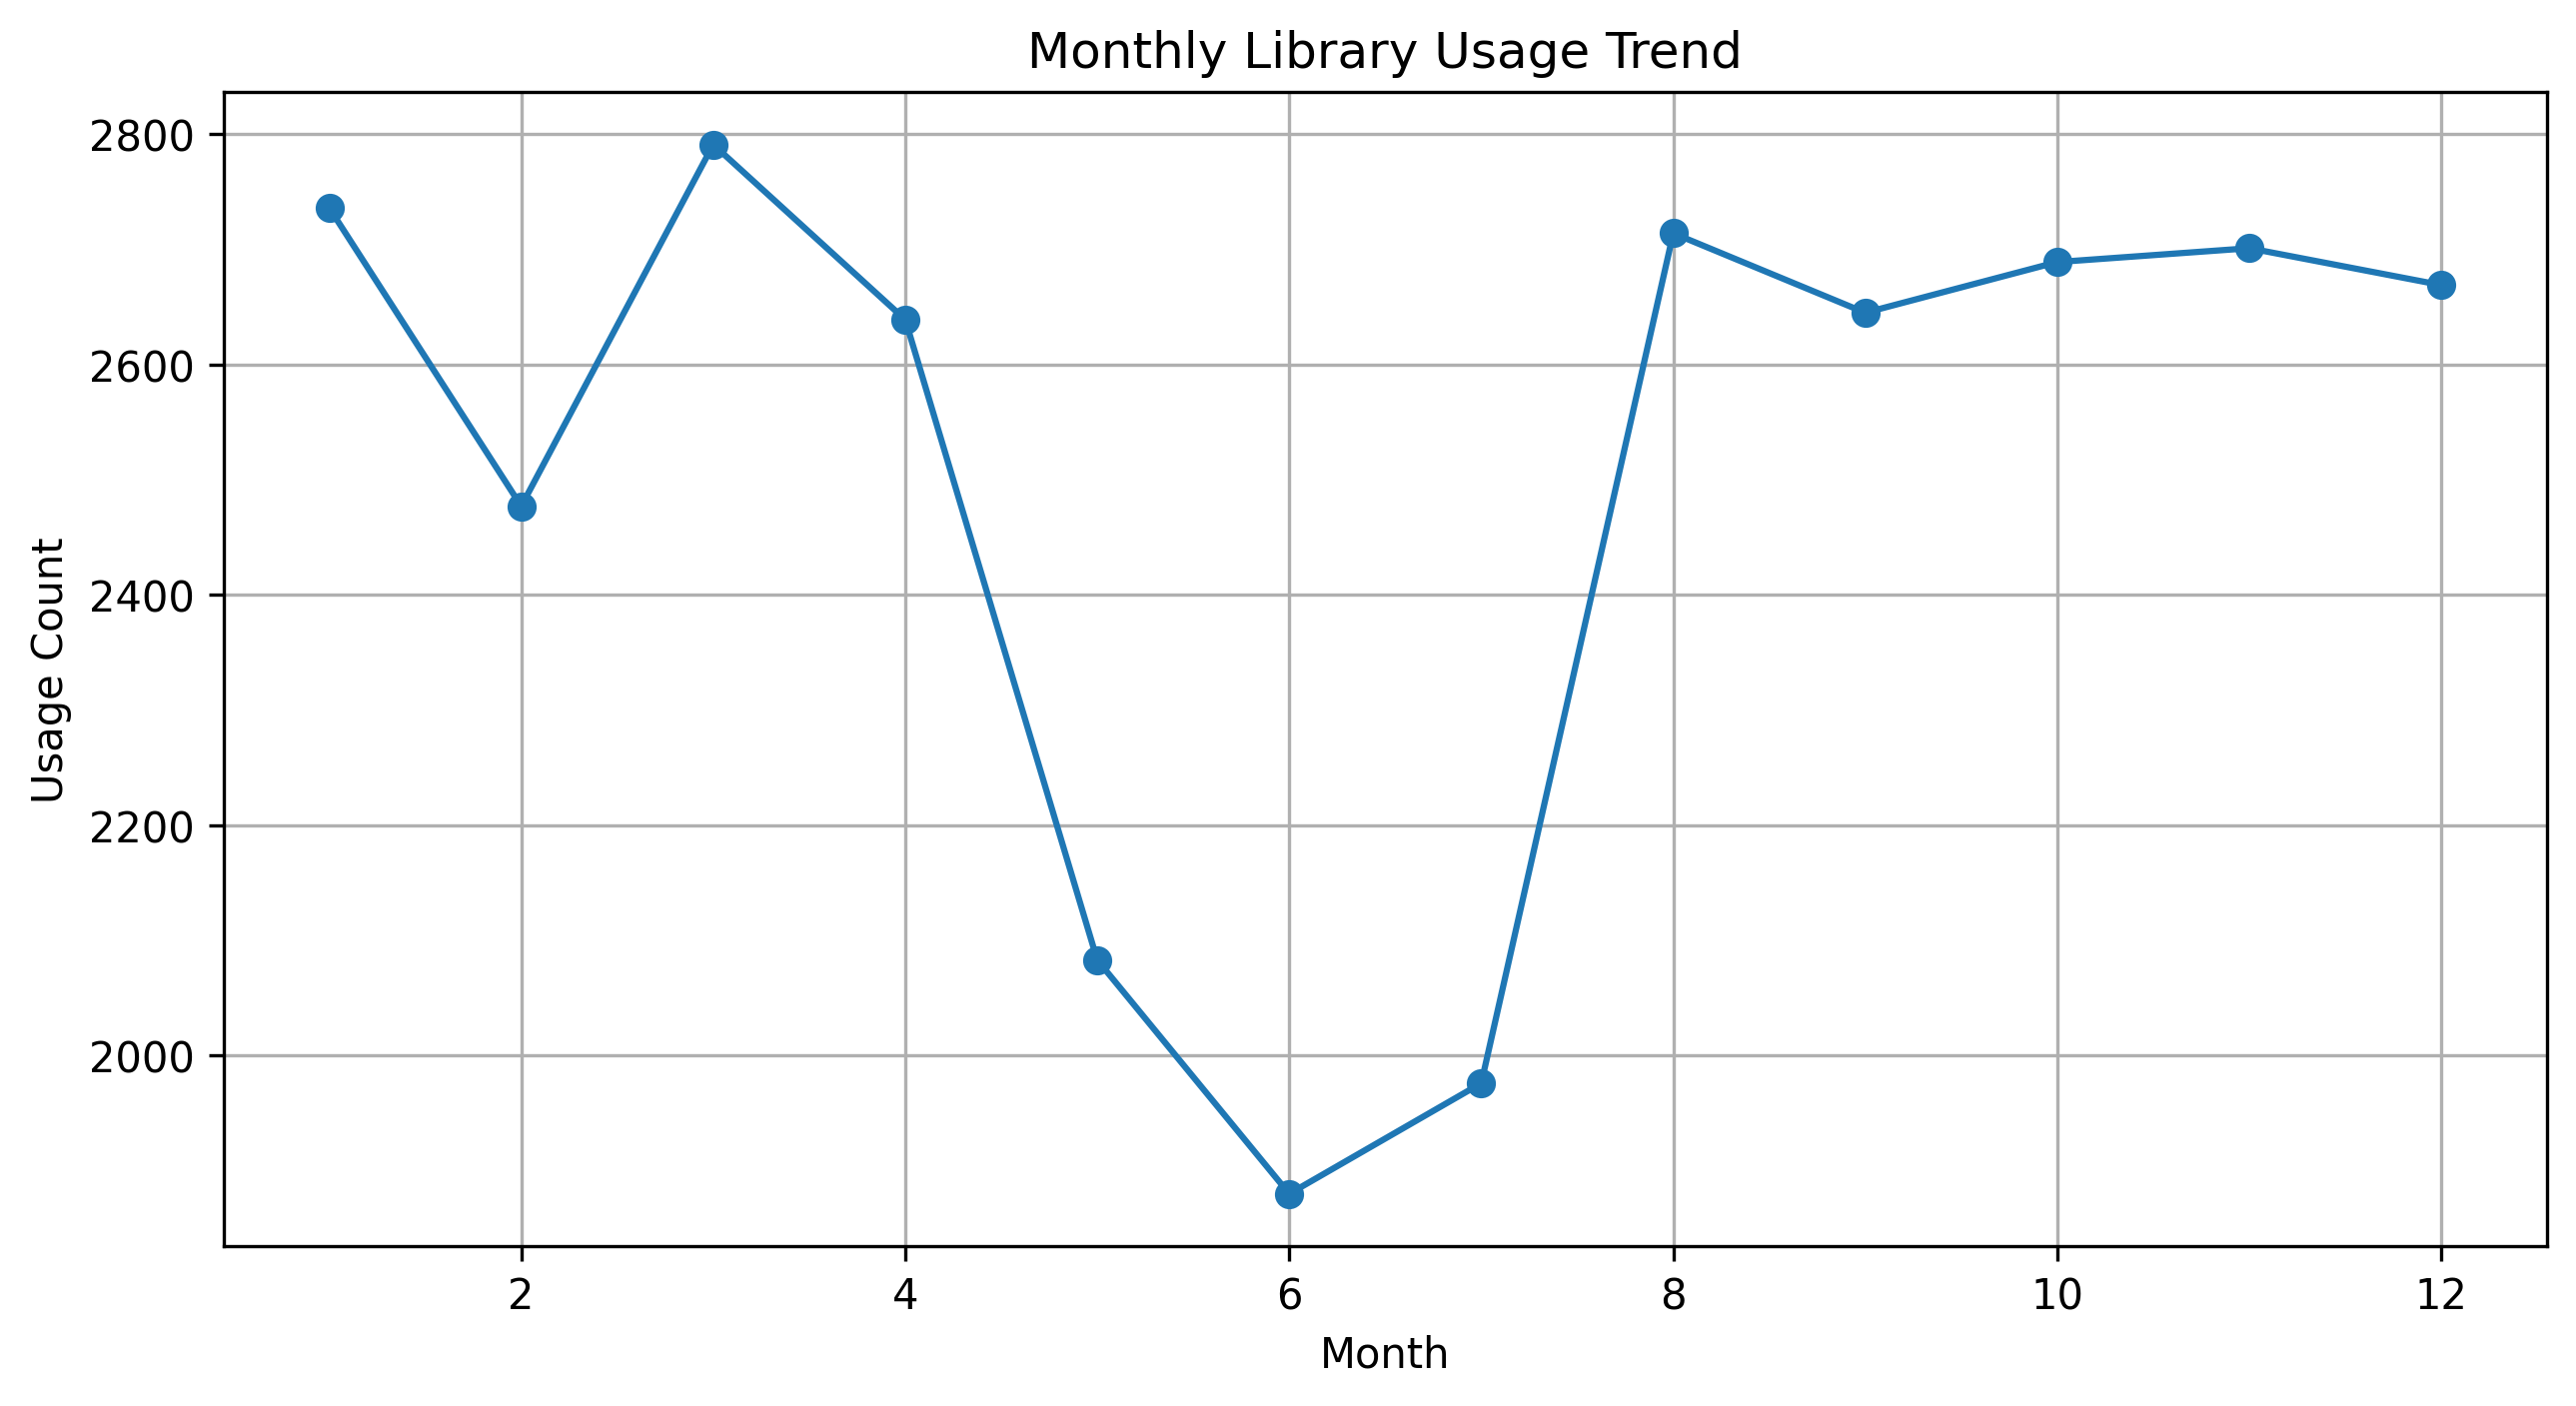
\includegraphics[width=0.9\textwidth]{saved_plots/plot_003_20260506_232423.png}
\caption{Monthly Library Usage Trend over the Year}
\end{figure}
\textit{Finding:} The peaks correspond directly with mid-term and end-term examination periods, where student footfall typically doubles.

\section{Peak Occupancy Hours}
Identifying the busiest hours of the day helps in managing library staff and facilities. The data shows that the library experiences peak occupancy between 13:00 and 15:00.

\begin{figure}[H]
\centering
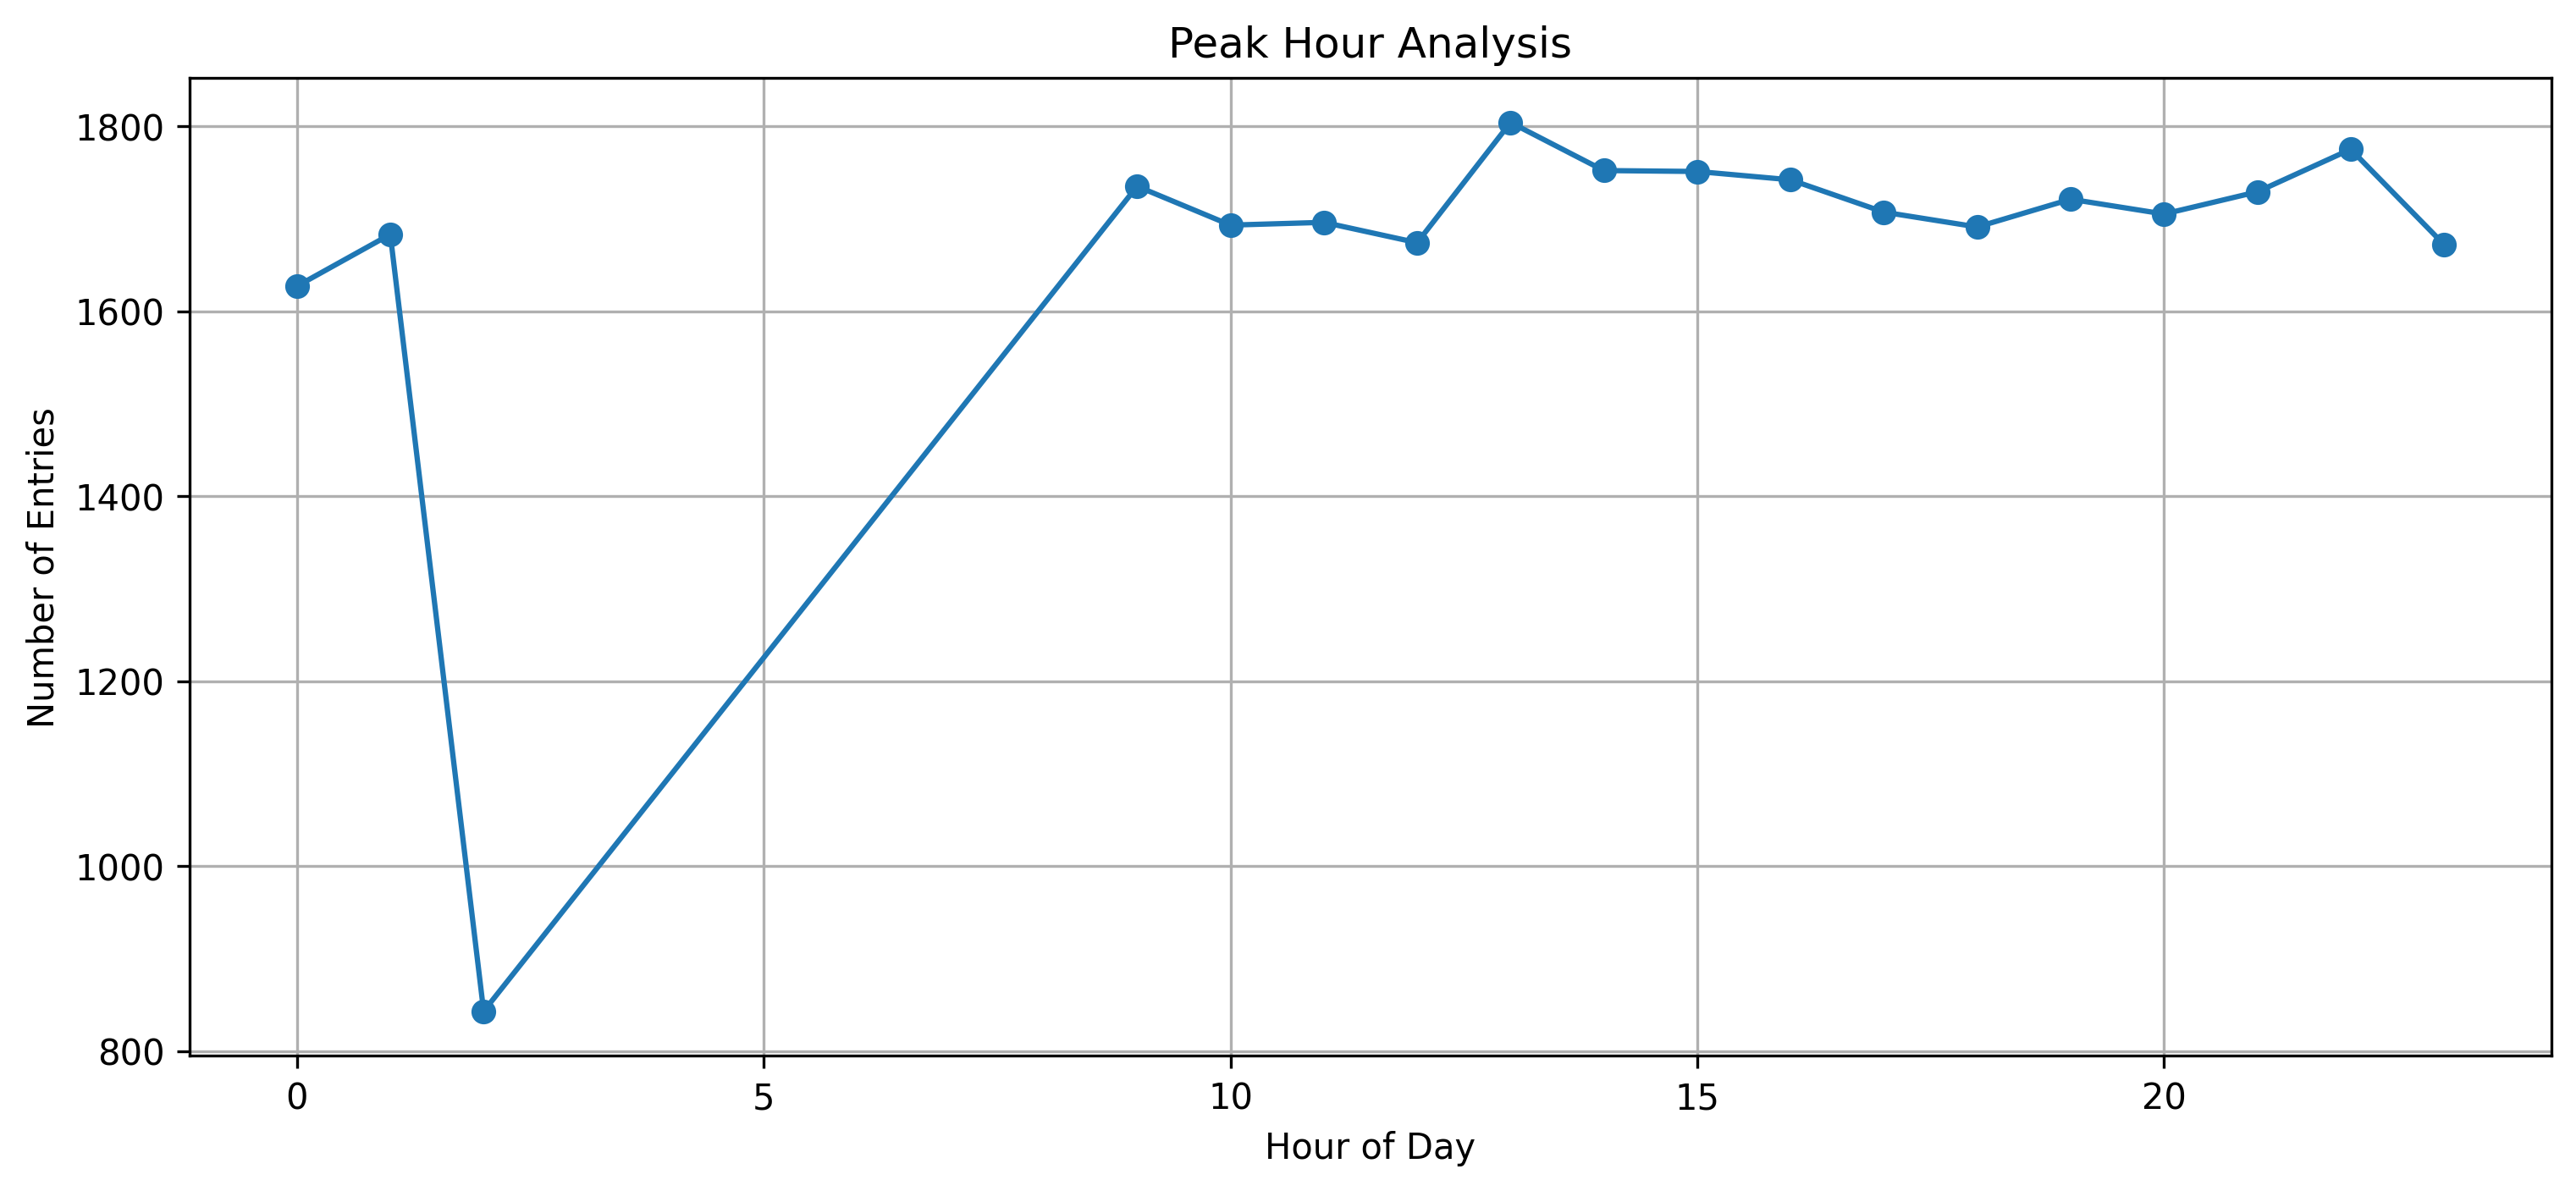
\includegraphics[width=0.9\textwidth]{saved_plots/plot_005_20260506_232424.png}
\caption{Hourly Library Entry Patterns (Peak Hours)}
\end{figure}
\textit{Finding:} Afternoon hours are the most crowded, suggesting that students prefer studying in the library after their morning classes.

\section{Correlation Analysis}
A correlation heatmap was generated to understand the relationship between different numerical variables like borrow duration, month, and entry hour.

\begin{figure}[H]
\centering
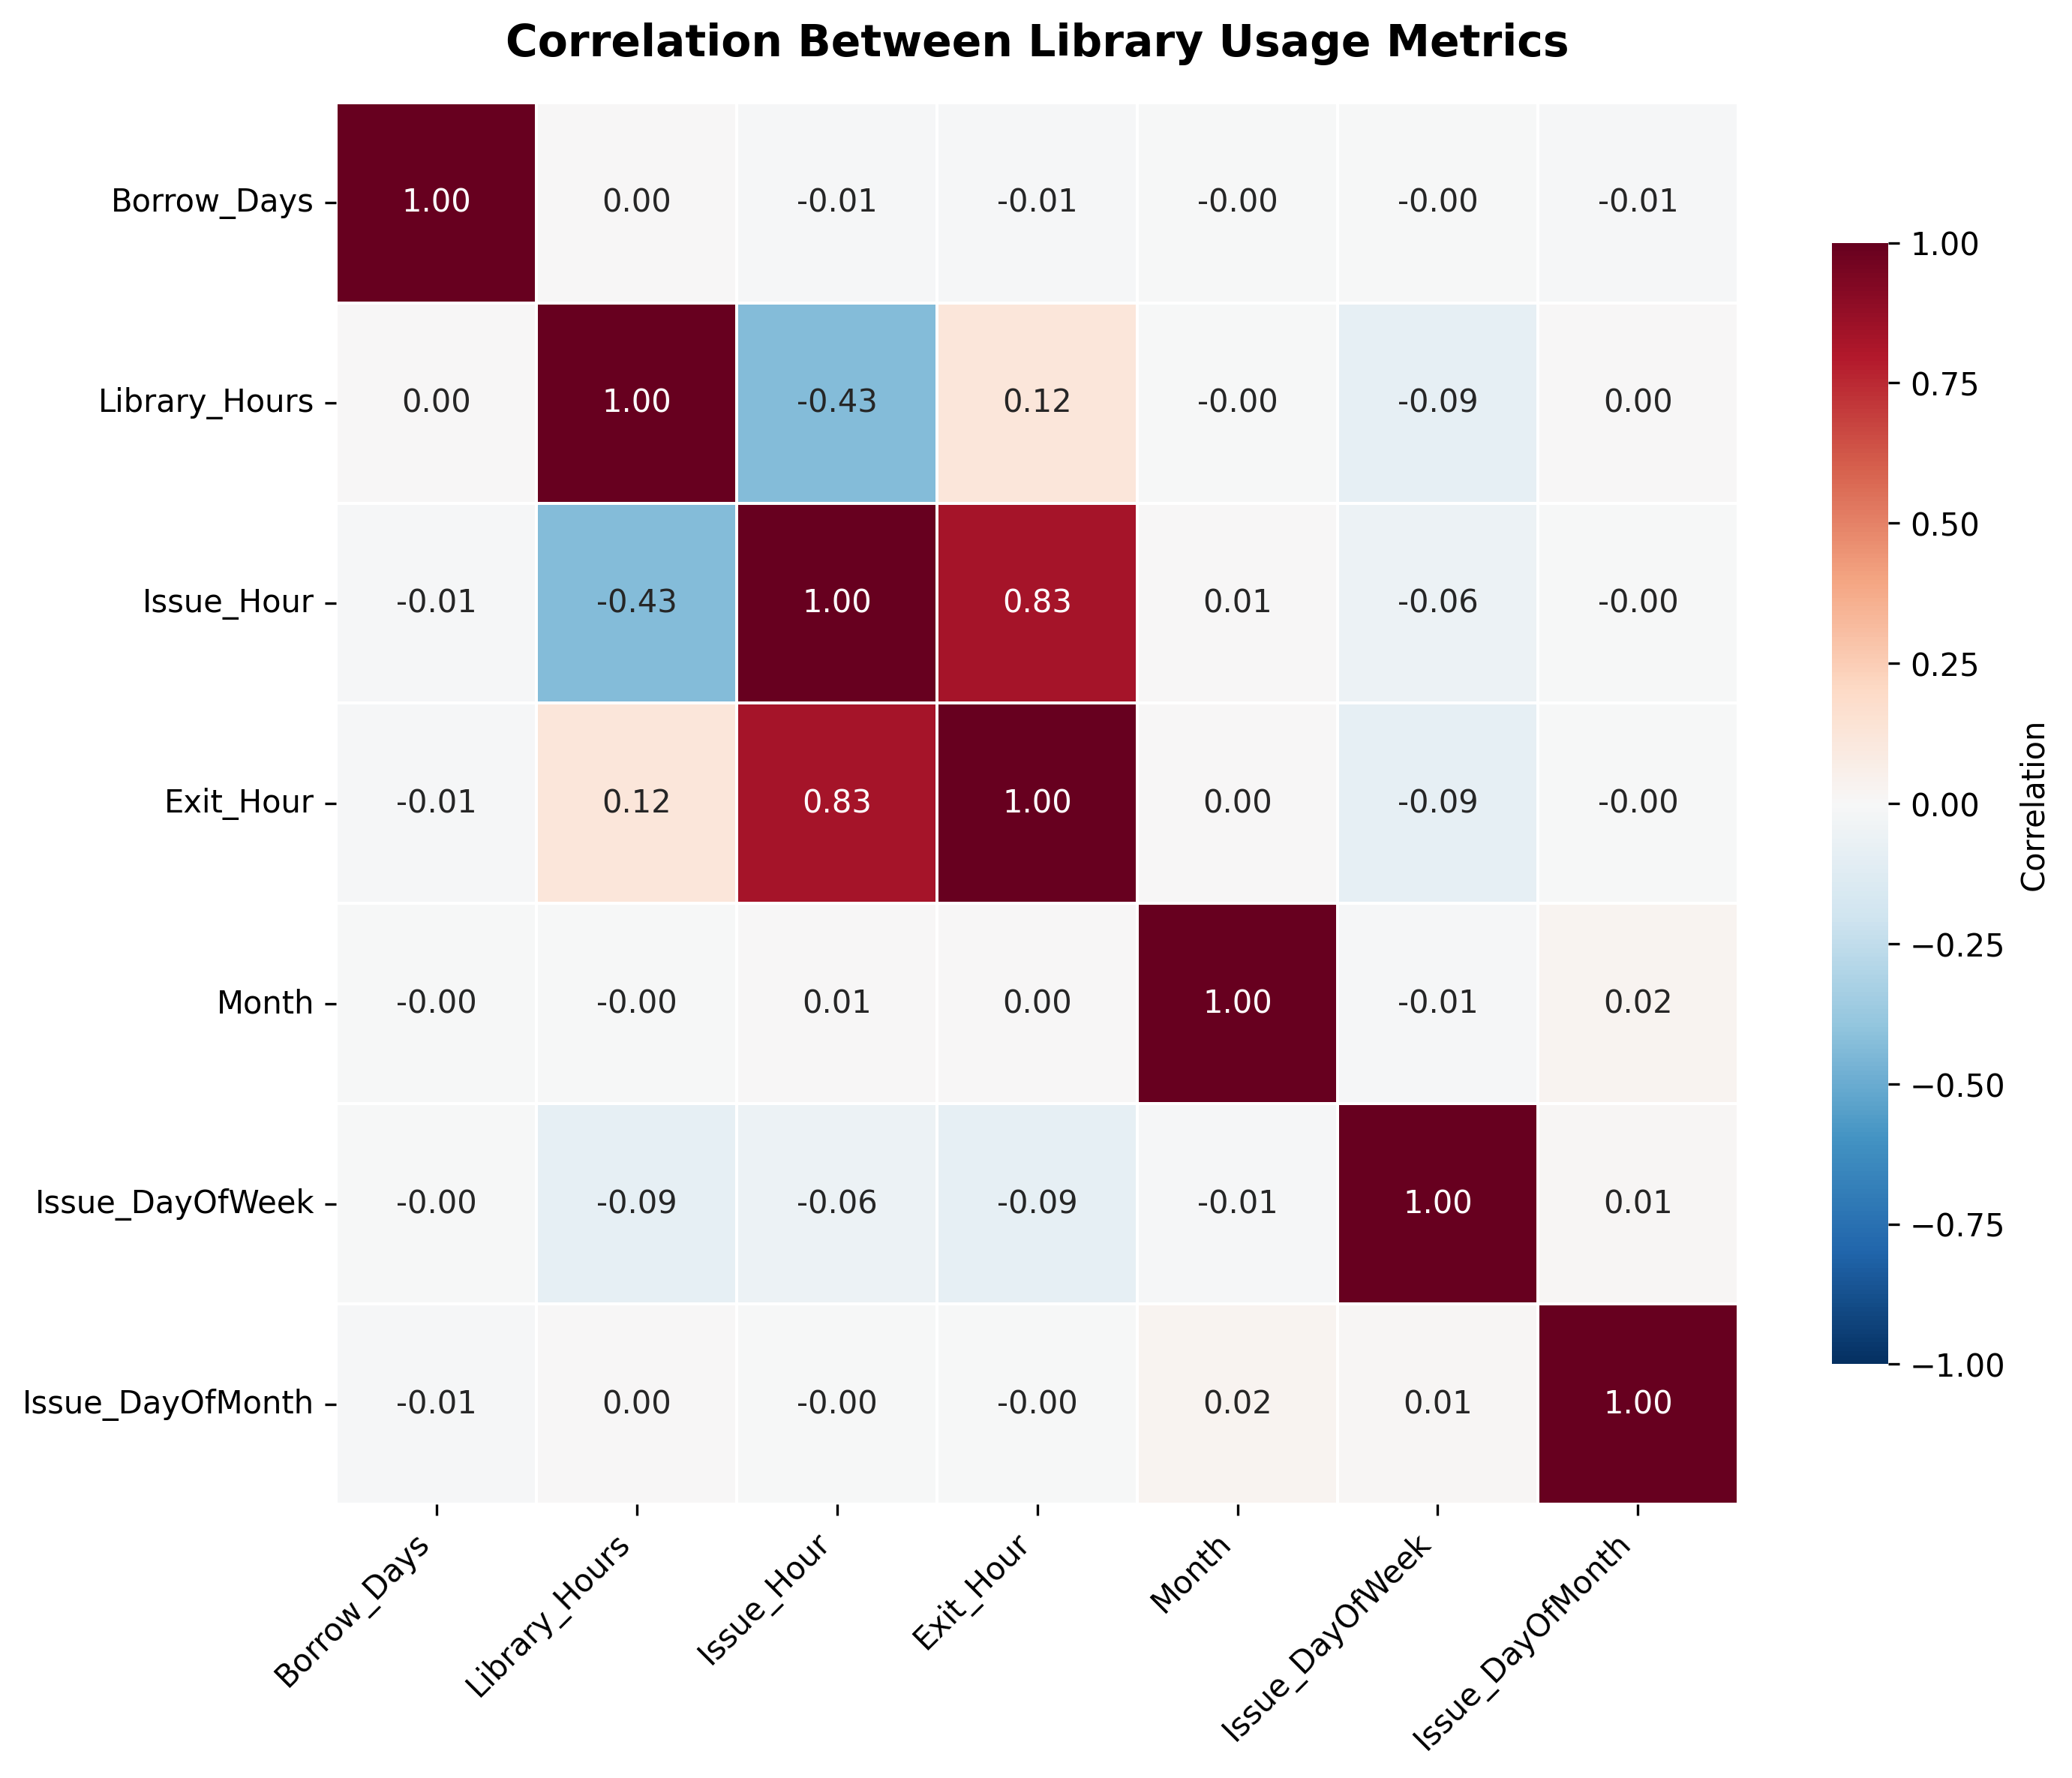
\includegraphics[width=0.85\textwidth]{saved_plots/plot_007_20260506_232425.png}
\caption{Correlation Heatmap of Library Usage Metrics}
\end{figure}
\textit{Finding:} While most variables showed weak correlations, the analysis helped in confirming that borrowing duration is relatively consistent regardless of the time of issue.

% ======================================================
% CHAPTER 7: DASHBOARD DEVELOPMENT
% ======================================================
\chapter{DASHBOARD DEVELOPMENT}
\section{Role of the Dashboard}
The final stage of the project involved the development of an interactive analytics dashboard. While stakeholders can use static charts for post-hoc analysis, a dashboard allows them to interact with the data, apply filters, and drill down into specific departments or categories. The dashboard serves as a "control tower" for library management.

\subsection{Dashboard Architecture}
The dashboard architecture defines the structural layout and the interactive components that constitute the user interface. It focuses on the hierarchy of information and the placement of analytical widgets to optimize the administrative user experience.

\begin{figure}[H]
\centering

\includegraphics[width=0.8\textwidth]{dashboard_architecture.png}
\caption{Dashboard Architecture and Interface Layout Design}
\label{fig:dashboard_arch}
\end{figure}

The architecture is composed of several interactive modules:
\begin{itemize}
    \item \textbf{Navigation Module (Sidebar):} Contains the department selectors, view mode switches (Global vs. Single Department), and data refresh status indicators.
    \item \textbf{KPI Summary Layer:} Positioned at the top, this layer uses stylized cards to present high-level metrics like total issues and engagement rates.
    \item \textbf{Comparative Analytics Layer:} Features bar charts and pie charts that allow for cross-departmental and category-wise comparisons.
    \item \textbf{Temporal Trend Layer:} Uses line charts to visualize historical usage patterns and seasonal variations.
    \item \textbf{Operational Layer:} Includes the data explorer table and export tools for manual record verification and reporting.
\end{itemize}

\subsection{Analytics Workflow Architecture}
The analytics workflow architecture represents the logical sequence of operations executed by the dashboard backend to generate real-time insights from the processed data.

\begin{figure}[H]
\centering

\includegraphics[width=0.85\textwidth]{analytics_workflow.png}
\caption{End-to-End Analytics Workflow and Insight Generation Logic}
\label{fig:workflow}
\end{figure}

The workflow follows a rigorous analytical path:
\begin{enumerate}
    \item \textbf{Data Initialization:} Loading the cleaned CSV files into memory using Pandas.
    \item \textbf{Dynamic Filtering:} Applying user-selected sidebar filters to the global dataframe to create local subsets of data.
    \item \textbf{Metric Computation:} Calculating averages and totals on-the-fly based on the filtered data.
    \item \textbf{Visualization Rendering:} Generating Plotly objects and Seaborn heatmaps dynamically.
    \item \textbf{Insight Delivery:} Rendering the final HTML elements and charts onto the Streamlit interface for the end-user.
\end{enumerate}

\section{Streamlit Framework}
Streamlit was chosen for its ability to turn Python scripts into interactive web apps. The dashboard is structured into several logical sections: KPI overview, department analysis, and temporal trends.

\subsection{User Interface Design}
The UI was designed to be clean and intuitive, following modern design principles. A sidebar allows users to switch between "All Departments" view and "Single Department" view. Custom CSS was injected into the Streamlit app to enhance the visual appeal, including gradient headers and stylized KPI cards.

\section{Power BI Dashboard Implementation}
In addition to the Streamlit application, a Power BI dashboard was developed to provide a more industrial-strength business intelligence solution. Power BI excels in handling complex data relationships and provides advanced interactive features that are highly effective for administrative reporting.

\subsection{Data Integration and Modeling}
The processed datasets, \textit{processed\_library\_data.csv} and \textit{processed\_study\_data.csv}, were imported into Power BI. A star-schema inspired data model was created to link library usage and study area records. DAX (Data Analysis Expressions) measures were implemented to calculate complex KPIs such as:
\begin{itemize}
    \item \textbf{Total Engagement:} A combined metric of book issues and study area visits.
    \item \textbf{Peak Utilization Rate:} Percentage of library occupancy during peak hours.
    \item \textbf{Return Compliance:} Ratio of books returned within the expected period.
\end{itemize}

\subsection{Interactive Visualizations}
The Power BI dashboard features multiple interactive pages:
\begin{itemize}
    \item \textbf{Executive Summary:} High-level view of library performance using cards and gauges.
    \item \textbf{Slicer-Driven Analysis:} Dynamic filtering by Department, Programme, and Time Period.
    \item \textbf{Cross-Highlighting:} Clicking on a specific department in a bar chart automatically filters all other visuals on the page to show data for that department.
\end{itemize}

\begin{figure}[H]
\centering
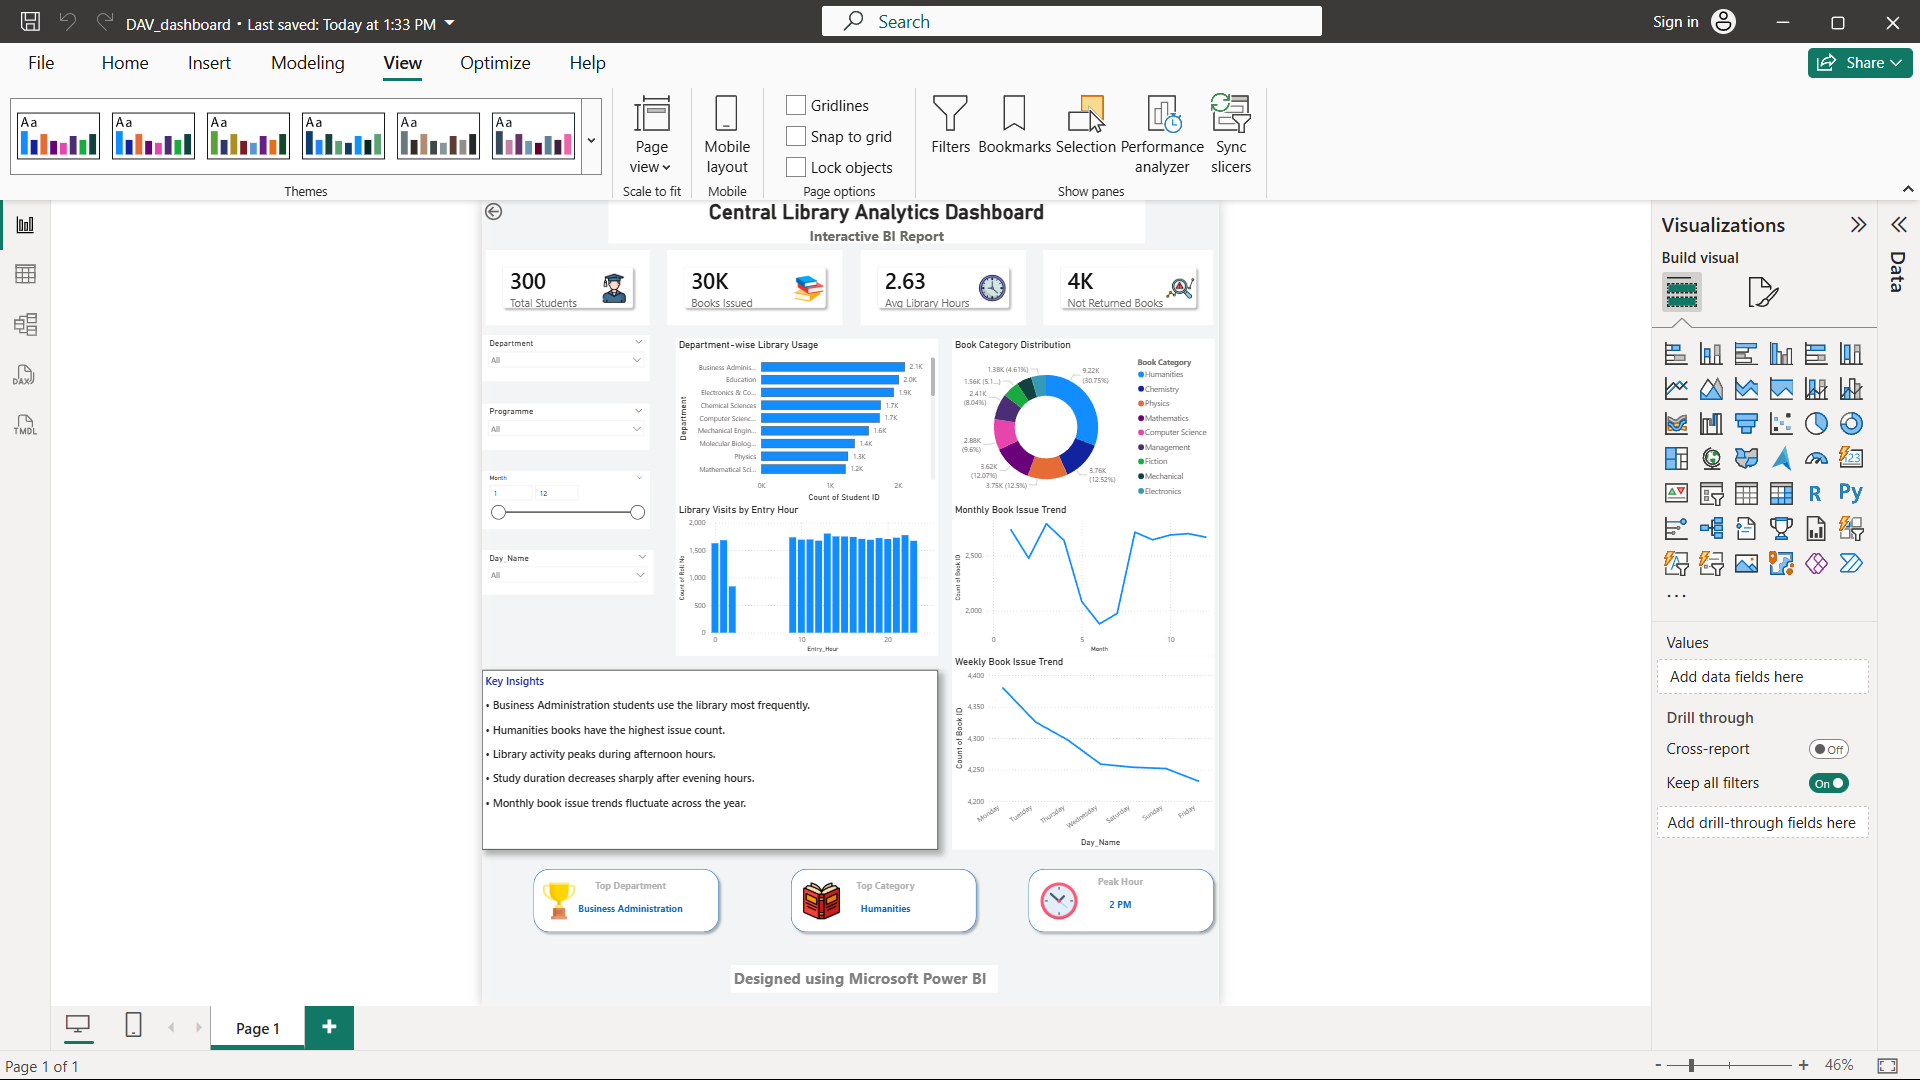
\includegraphics[width=0.9\textwidth]{powerbi_dashboard.png}
\caption{Power BI Administrative Analytics Interface}
\end{figure}
\FloatBarrier

\section{Key Features of the Dashboard}
\begin{itemize}
    \item \textbf{KPI Cards:} Provide immediate metrics like total books issued, average borrow days, and unique students.
    \item \textbf{Department Search:} A real-time search filter for quick navigation through dozens of academic branches.
    \item \textbf{Interactive Charts:} Built using Plotly, these charts allow users to hover for details and zoom into specific data points.
    \item \textbf{Data Explorer:} A table view at the bottom of the dashboard allowing for manual inspection of records.
    \item \textbf{Export Functionality:} Allows administrators to download filtered data as CSV files for further reporting.
\end{itemize}

\begin{lstlisting}[language=Python, caption=Dashboard KPI Implementation]
# Calculate KPI metrics
total_books = len(filtered_library)
avg_borrow = round(filtered_library['Borrow_Days'].mean(), 2)
avg_study = round(filtered_study['Study_Duration_Hours'].mean(), 2)

# Displaying KPI in Streamlit
col1, col2, col3 = st.columns(3)
col1.metric("Books Issued", total_books)
col2.metric("Avg Borrow Days", avg_borrow)
col3.metric("Avg Study Hours", avg_study)
\end{lstlisting}

\section{Visualization Logic}
The dashboard utilizes \textit{Plotly Express} for generating dynamic visualizations. For example, the department usage chart automatically updates its ranking based on the global or filtered dataset. The monthly trend chart uses a line-with-markers mode to highlight seasonal fluctuations.

% ======================================================
% CHAPTER 8: RESULTS AND DISCUSSION
% ======================================================
\chapter{RESULTS AND DISCUSSION}
\section{Summary of Findings}
The comprehensive analysis of the library datasets yielded several significant insights into student behavior and resource utilization.
\begin{itemize}
    \item \textbf{High-Volume Departments:} Business Administration, Education, and ECE are the primary drivers of library footfall. This suggests that students in these fields rely heavily on library-maintained reference materials.
    \item \textbf{Resource Preferences:} The strong preference for "Humanities" and "Core Science" books suggests that despite the digital shift, physical textbooks remain foundational to university education.
    \item \textbf{Temporal Patterns:} The sharp increase in usage during end-of-semester months confirms the library's role as a critical study environment during exam seasons.
    \item \textbf{Study Habits:} The average study duration per session varies across departments, with engineering students generally spending longer continuous hours in the study area.
\end{itemize}

\section{Institutional Implications}
The findings have direct implications for institutional resource planning.
\begin{itemize}
    \item \textbf{Staffing:} Library staffing should be increased by approximately 30\% during the peak 13:00--15:00 window.
    \item \textbf{Procurement:} Funds should be prioritized for categories with the highest turnover rates, such as Management and Computer Science.
    \item \textbf{Space Management:} Given the high occupancy rates during exams, the institution might consider converting adjacent classrooms into temporary study halls during these peak periods.
\end{itemize}

\section{Technical Discussion}
The use of Python for preprocessing and Streamlit for the dashboard proved to be a highly efficient workflow. The system was able to process 60,000 records with sub-second latency, demonstrating its scalability. The interactive nature of Plotly charts significantly improved the "explorability" of the data compared to static Matplotlib plots.

\section{Team Contribution}
The University Central Library Analytics project was executed through a highly collaborative and iterative workflow, ensuring seamless integration between data engineering, exploratory analysis, and interactive visualization modules. The division of work was strategically planned to maintain technical consistency while allowing for specialized development in both the Python-based analytical stack and the Business Intelligence dashboard frameworks. Systematic coordination and regular synchronization meetings allowed the team to track technical contributions in real-time, ensuring that the insights derived from the Exploratory Data Analysis were accurately translated into the final interactive dashboards. This collaborative synergy was instrumental in transforming over 60,000 raw transaction logs into a professional-grade administrative reporting system.

\begin{table}[H]
\centering
\small
\begin{tabularx}{\textwidth}{@{}|X|X|@{}}
\hline
\rowcolor[HTML]{EFEFEF} 
\textbf{Member 1 Contribution (Akashdeep Singha)} & \textbf{Member 2 Contribution (Udoyan Ojah)} \\ \hline
Meticulous collection and organization of the library usage and study area transaction datasets to ensure structural integrity. & Design and development of the full-stack Streamlit web application architecture for real-time data interaction. \\ \hline
Implementation of robust data preprocessing pipelines using Python and Pandas for systematic cleaning of raw administrative logs. & Creation of the industrial-strength Power BI dashboard for advanced administrative business intelligence reporting. \\ \hline
Comprehensive handling of missing values and noise reduction across 60,000 records to improve statistical accuracy. & Strategic implementation of interactive KPI cards to provide immediate visibility into critical library performance metrics. \\ \hline
Advanced date and time conversion from string formats into Python datetime objects to enable longitudinal analysis. & Integration of dynamic donut charts and Plotly-based visualizations to showcase resource distribution across departments. \\ \hline
Detailed feature engineering, including the derivation of new metrics such as Borrow\_Days and Study\_Duration\_Hours. & User Interface (UI) design and layout optimization to ensure an intuitive and professional user experience across platforms. \\ \hline
Exhaustive Exploratory Data Analysis (EDA) to uncover hidden patterns in student engagement and resource utilization. & Validation of all visualizations against processed datasets to ensure absolute data consistency and reporting accuracy. \\ \hline
Statistical analysis and correlation studies using Seaborn to identify relationships between different usage variables. & Technical organization and formatting of the LaTeX project report to meet professional academic submission standards. \\ \hline
Full implementation of the analytical logic in Jupyter Notebooks, serving as the technical foundation for the project. & Integration of multi-platform screenshots and preparation of comprehensive presentation materials for the project viva. \\ \hline
Extraction of actionable academic insights and validation of data patterns to provide institutional recommendations. & Collaborative testing of dashboard filters and slicers to ensure a bug-free and responsive analytical environment. \\ \hline
\end{tabularx}
\caption{Detailed Project Contribution and Work Distribution Matrix}
\label{table:contribution}
\end{table}
\FloatBarrier

% ======================================================
% CHAPTER 9: CONCLUSION AND FUTURE WORK
% ======================================================
\chapter{CONCLUSION AND FUTURE WORK}
\section{Conclusion}
This project successfully demonstrated the application of data analytics and visualization in an institutional setting. By transforming raw library logs into a comprehensive analytics dashboard, we have provided a tool that enhances administrative oversight and resource optimization. The project journey, from data cleaning to interactive visualization, highlights the power of the Python ecosystem in solving real-world operational challenges. The insights gained regarding peak hours, popular book categories, and departmental usage patterns offer a solid foundation for evidence-based library management.

\section{Learning Outcomes}
Through this project, several key technical and professional skills were acquired:
\begin{itemize}
    \item Advanced data manipulation using Pandas and NumPy.
    \item Statistical visualization using Seaborn and Plotly.
    \item Web-based application development using Streamlit.
    \item Academic technical writing and research documentation.
\end{itemize}

\section{Future Work}
While the current system provides robust analytical capabilities, there are several avenues for future enhancement:
\begin{itemize}
    \item \textbf{Predictive Modeling:} Implementing Machine Learning models to predict future book demand and occupancy spikes.
    \item \textbf{Real-time RFID Integration:} Connecting the dashboard to a live RFID stream for instantaneous footfall tracking.
    \item \textbf{Recommendation System:} Developing a personalized book recommendation engine for students based on their borrowing history.
    \item \textbf{Sentiment Analysis:} Analyzing student feedback and reviews to improve library services.
\end{itemize}

% ======================================================
% REFERENCES
% ======================================================
\newpage
\begin{thebibliography}{99}
\bibitem{ref1} W. McKinney, "Python for Data Analysis: Data Wrangling with Pandas, NumPy, and IPython," O'Reilly Media, 2017.
\bibitem{ref2} J. Hunter, "Matplotlib: A 2D Graphics Environment," Computing in Science \& Engineering, 2007.
\bibitem{ref3} M. Waskom, "Seaborn: Statistical Data Visualization," Journal of Open Source Software, 2021.
\bibitem{ref4} Streamlit Documentation, "The Fastest Way to Build Data Apps," [Online]. Available: https://docs.streamlit.io.
\bibitem{ref5} A. Sievert and C. Shirley, "LDAvis: A method for visualizing and interpreting topics," Proceedings of the workshop on interactive language learning, visualization, and interfaces, 2014.
\bibitem{ref6} IEEE Standard for Software Test Documentation, "IEEE Std 829-2008," 2008.
\end{thebibliography}

% ======================================================
% APPENDIX
% ======================================================
\chapter*{APPENDIX}
\addcontentsline{toc}{chapter}{APPENDIX}
\section*{Important Code Snippets}
\begin{lstlisting}[language=Python, caption=Data Export Script]
# Exporting the final processed datasets
library_df.to_csv("processed_library_data.csv", index=False)
study_df.to_csv("processed_study_data.csv", index=False)
\end{lstlisting}

\section*{Dashboard Screenshot Gallery}
\begin{figure}[H]
\centering
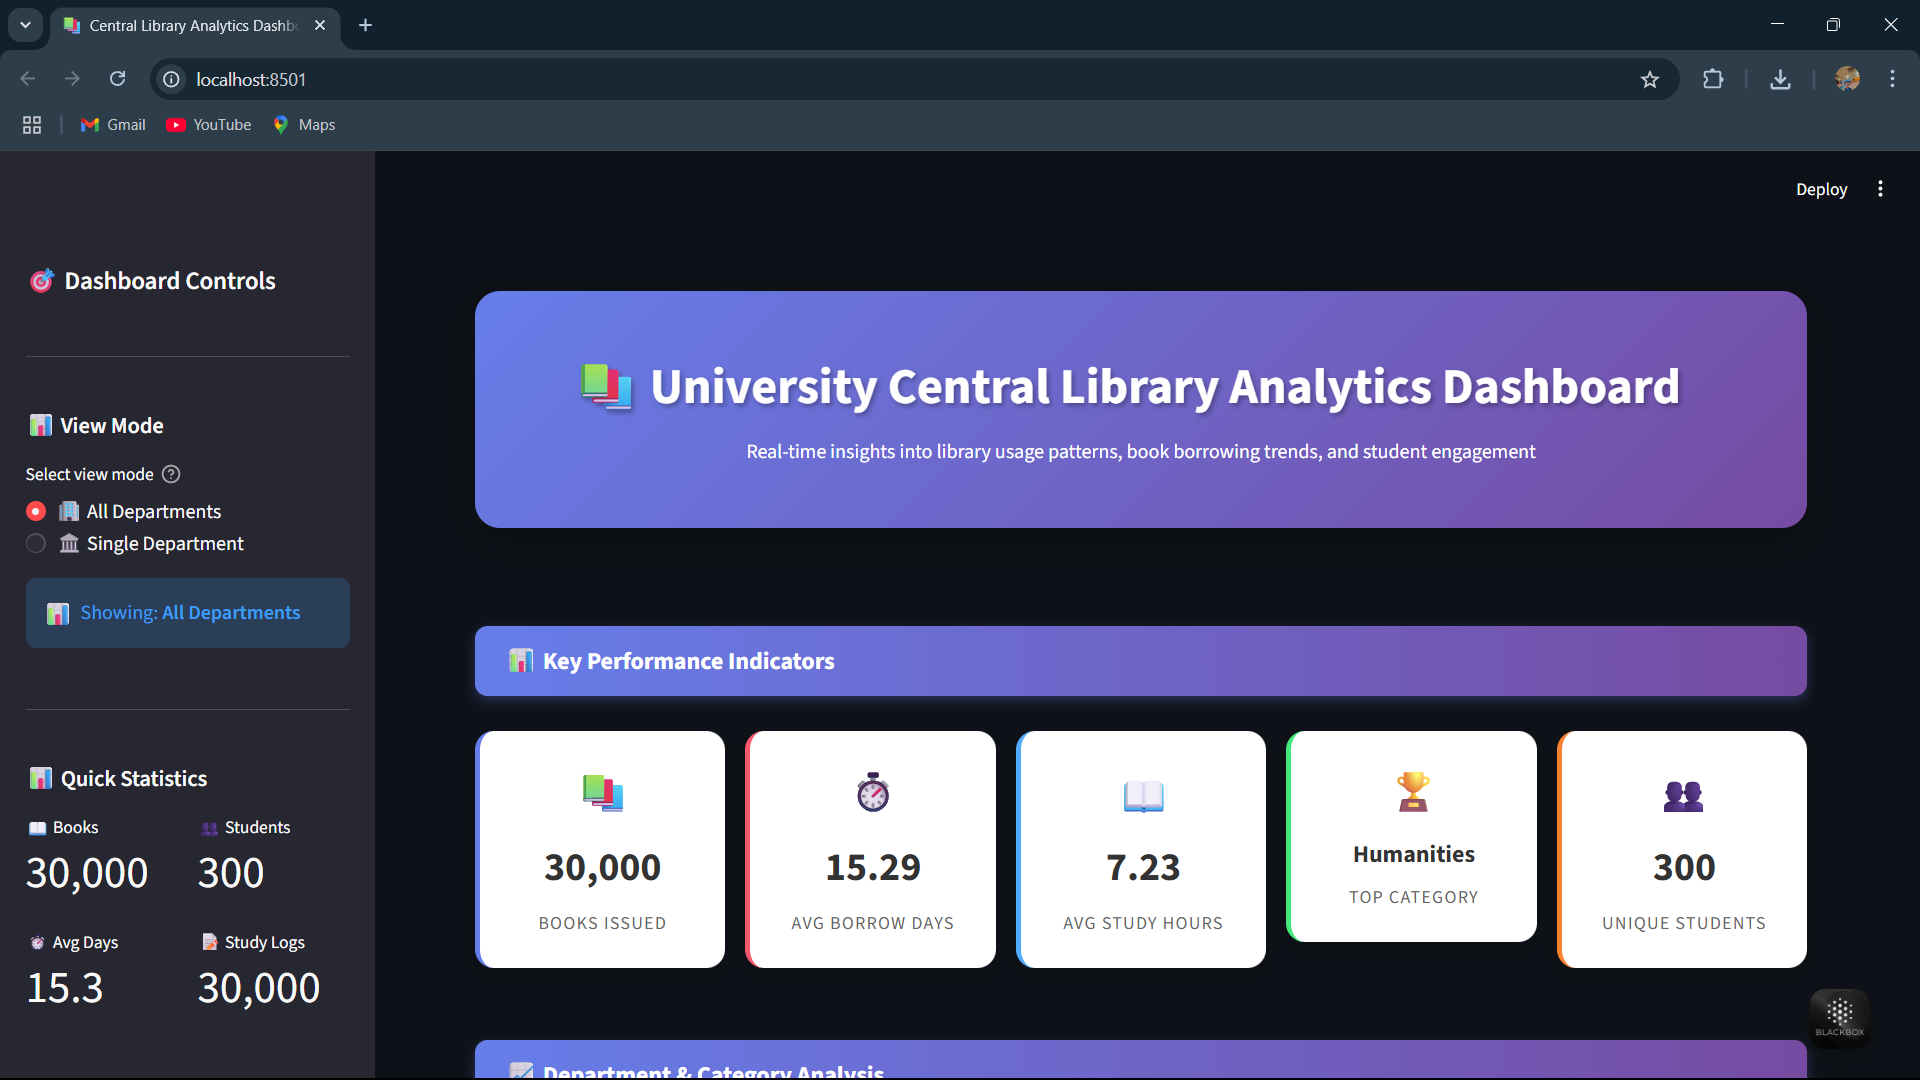
\includegraphics[width=\textwidth]{dashboard_kpi.png}
\caption{Main Overview Dashboard with KPI Cards}
\end{figure}

\begin{figure}[H]
\centering
\includegraphics[width=\textwidth]{dashboard_categories.png}
\caption{Category Distribution and Global Trends Analysis}
\end{figure}

\begin{figure}[H]
\centering
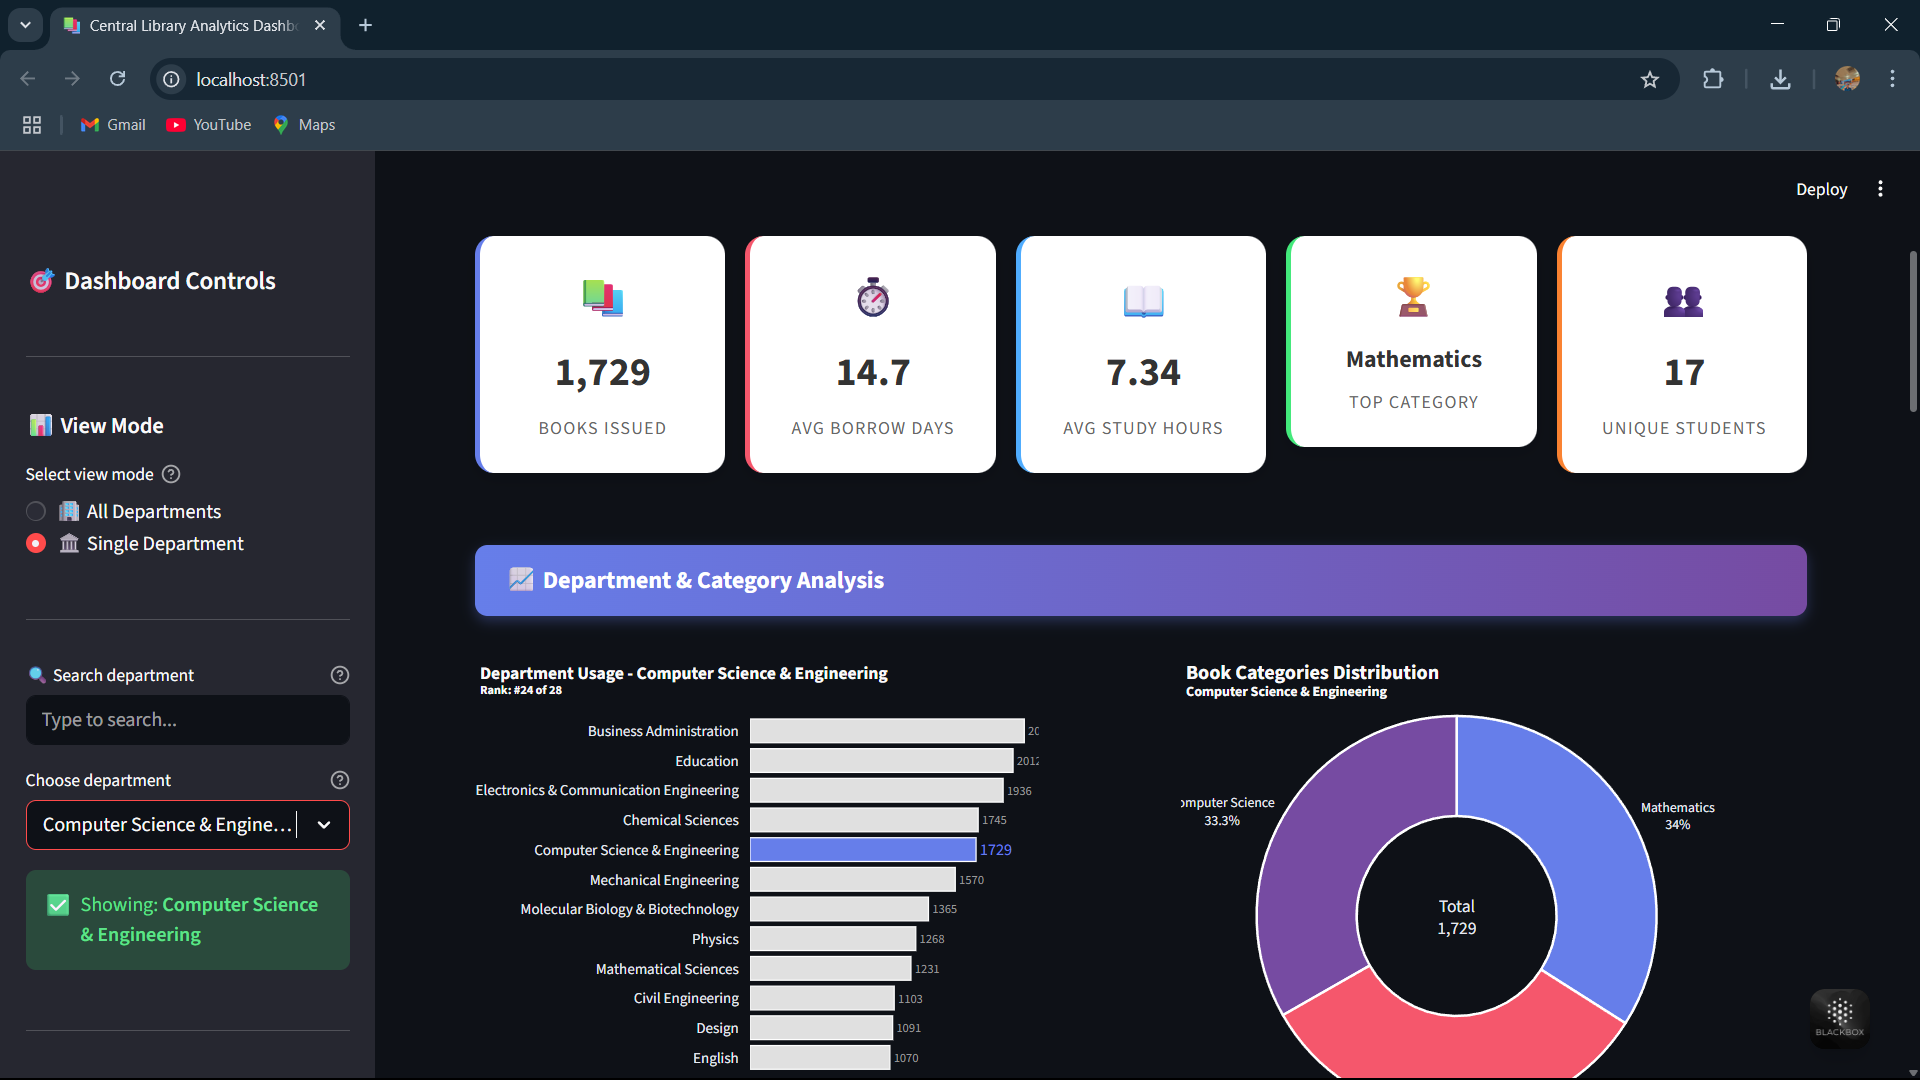
\includegraphics[width=\textwidth]{dashboard_filtering.png}
\caption{Interactive Department-wise Filtering and Comparative Metrics}
\end{figure}

\begin{figure}[H]
\centering
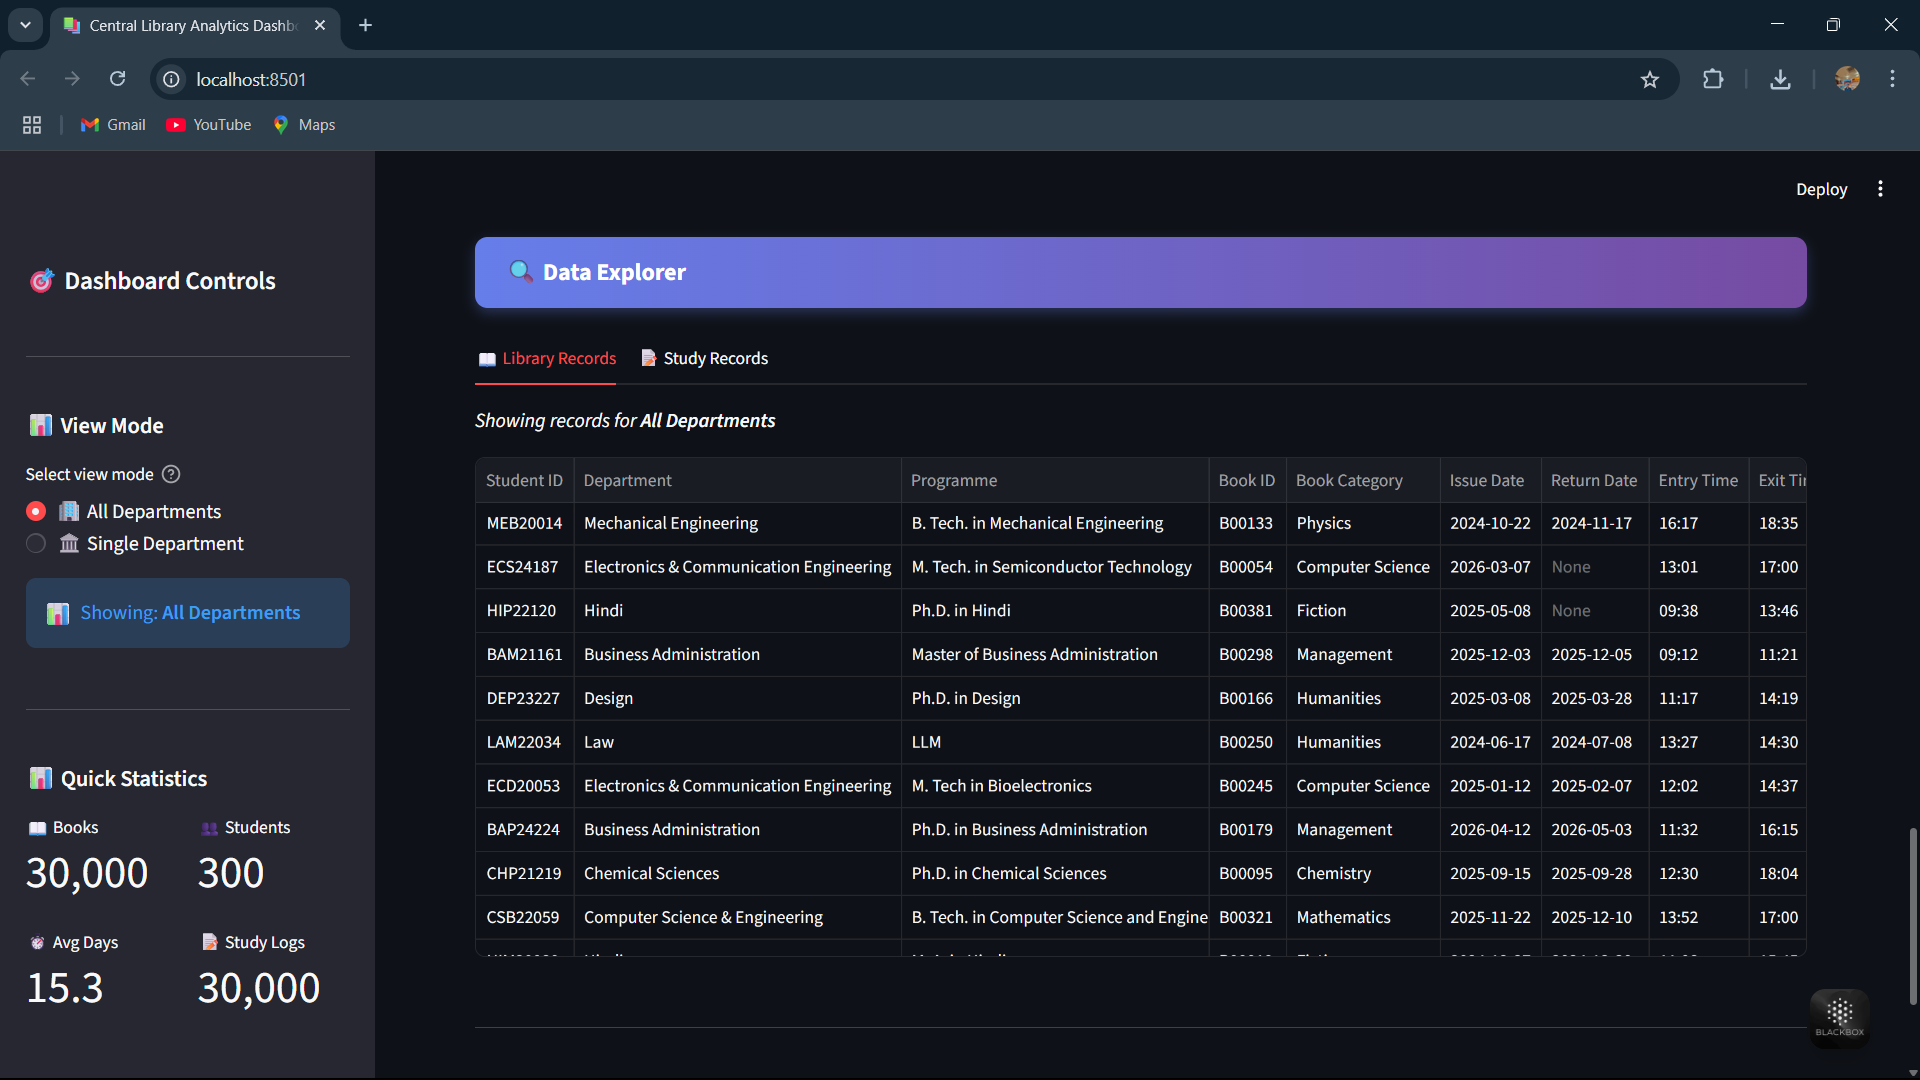
\includegraphics[width=\textwidth]{dashboard_data.png}
\caption{Data Explorer Interface and Administrative Filters}
\end{figure}

\begin{figure}[H]
\centering
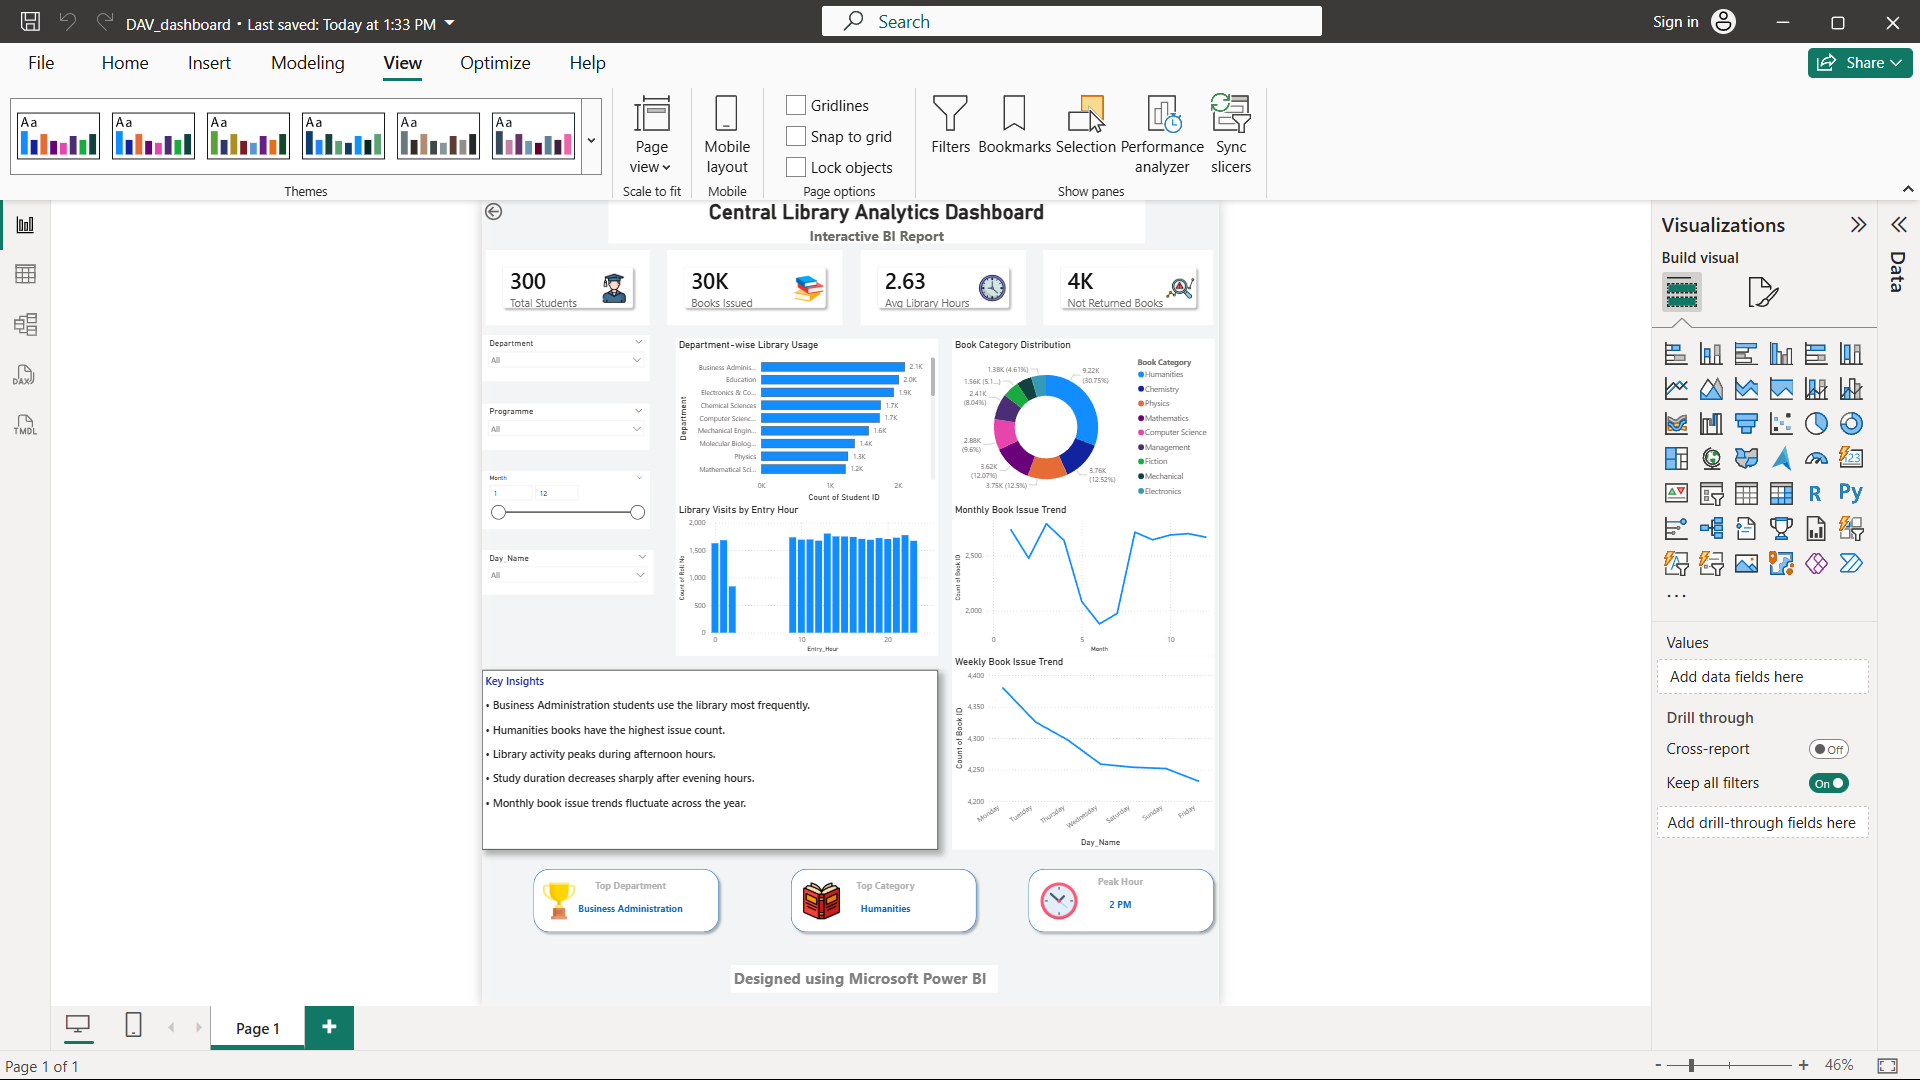
\includegraphics[width=\textwidth]{powerbi_dashboard.png}
\caption{Power BI Administrative Analytics Interface - Detailed View}
\end{figure}

\end{document}
